\section{Data Processing}
\label{sec:data-processing}

\subsection{Trigger}
As described in section \ref{sec:dom-daq}, the high-frequency ATWD waveform digitization in each DOM is triggered when it and its adjacent or next-to-adjacent neighbors on the same string record a voltage of at least 0.25 PE-equivalent within a $\pm$1~$\mu$s time window, which is referred to as the Hard Local Coincidence (HLC) condition. Data acquisition for DeepCore is triggered when this condition is fulfilled for at least three DOMs inside the DeepCore fiducial volume within a $\pm$2.5~$\mu$s window. If this condition is met, the waveforms for all DOMs that have observed voltages of at least 0.25~PE within a $\pm$10~$\mu$s time window centered around the trigger time are recorded. A DOM that is included in this readout but for which the HLC condition has not been met is said to fulfill the \emph{Soft Local Coincidence} (SLC) condition. The DeepCore trigger rate is less than 10~Hz and will trigger on \~70\% of $\nu_\mu$ events at 10~GeV and >90\% of $\nu_\mu$ events at 100~GeV\cite{DeepCore}.

\subsection{Online Filter}

Once the trigger condition is met, the recorded waveforms within the trigger window are converted into reconstructed pulses and are then passed into a set of \emph{online} filters (i.e. filters running on hardware at the Pole). These filters are each designed to select events that are relevant to different physics measurements that are performed within the IceCube collaboration. For the purposes of the analysis presented in this thesis, events are selected using the \emph{DeepCore filter}. This filter is designed to select events that start inside the DeepCore fiducial volume and to reject those that are consistent with muons entering the detector from the outside.
\begin{marginfigure}
    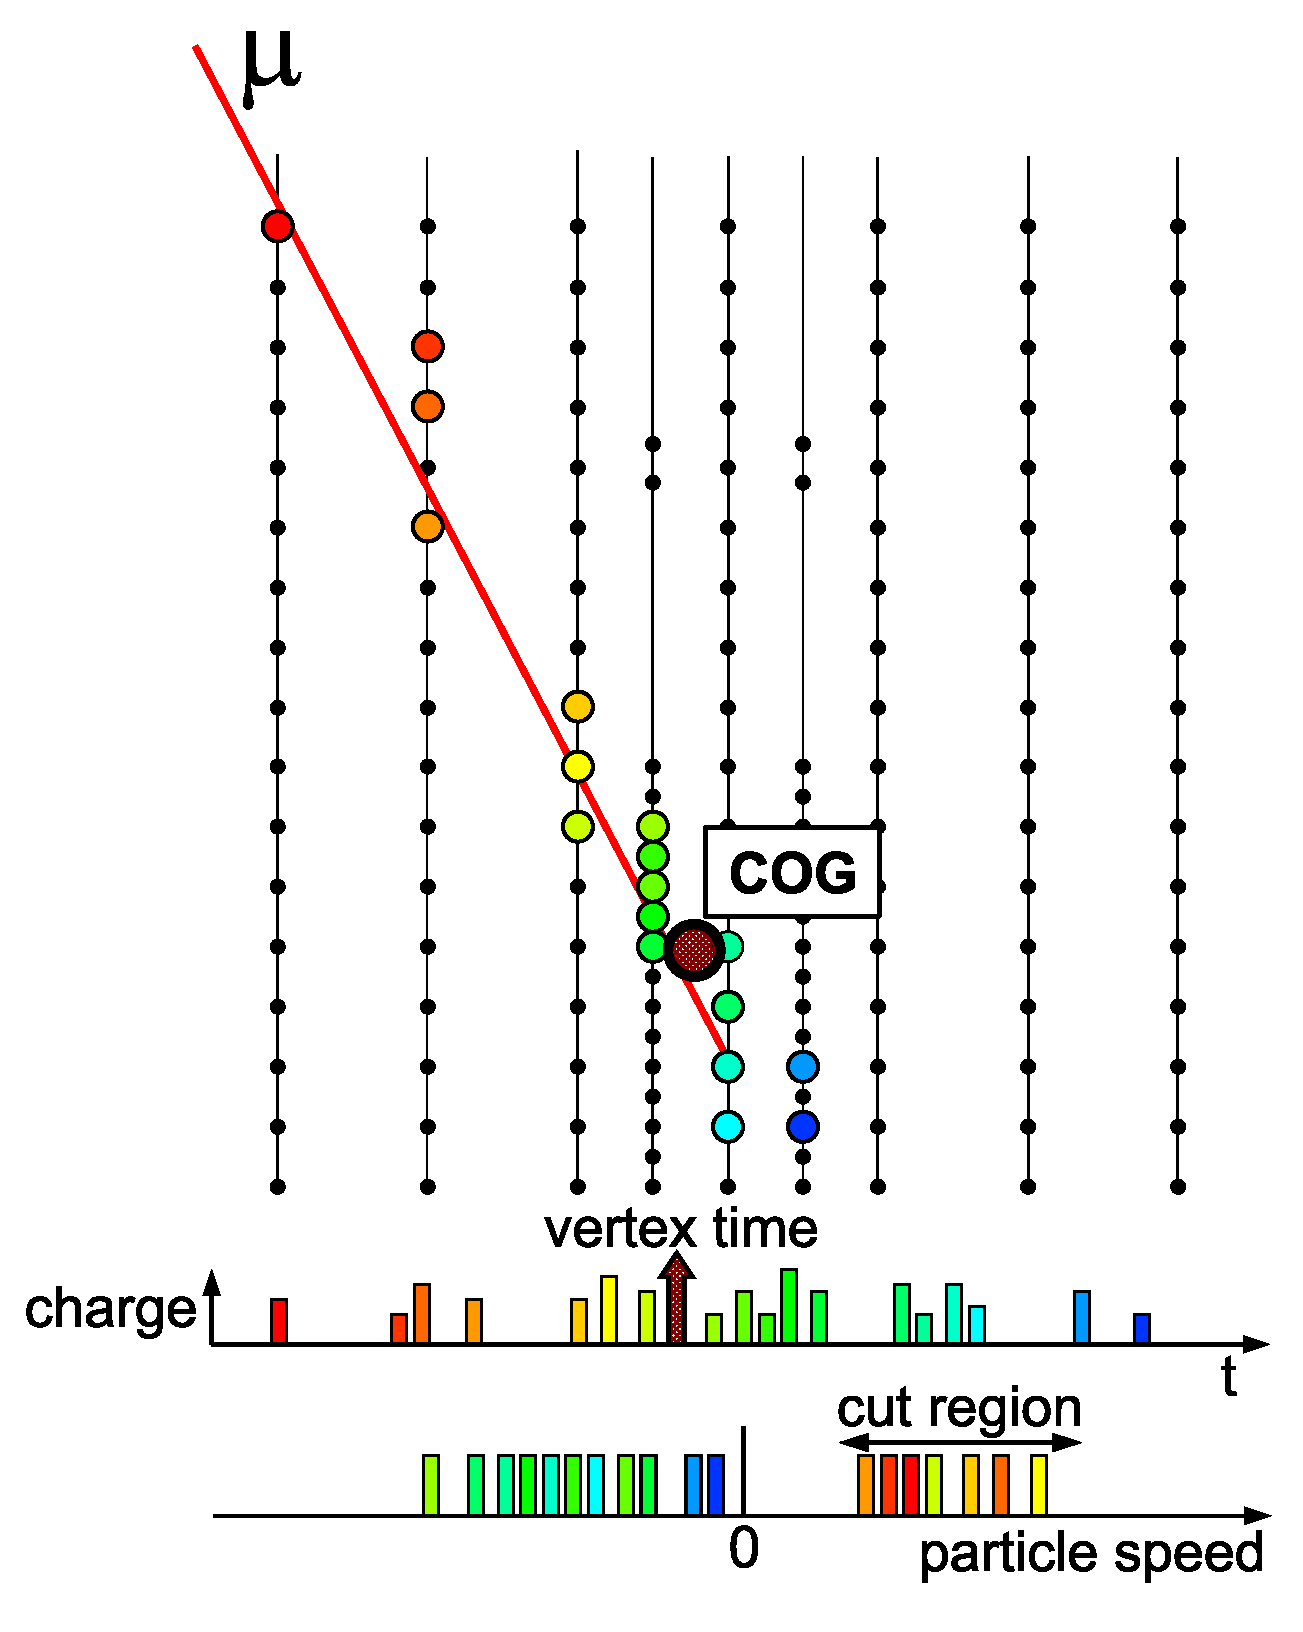
\includegraphics[width=\textwidth]{figures/icecube/eventviews/FilterDiagram.pdf}
    \caption{Example of an event that would be rejected by the online filter algorithm. DOMs that have observed light are highlighted in color depending on time from red (early hits) to blue (late hits). DOMs that have not observed any light are shown as black dots. Figure taken from \cite{DeepCore}.}
    \label{fig:online-filter-event}
\end{marginfigure}
The filter first applies a noise cleaning algorithm based on a coincidence condition between hits on different DOMs, where hits in DOMs for which the HLC condition was met are always kept. The cleaned hit series is split between those hits that fall within the DeepCore fiducial volume and those outside of it. The veto algorithm then calculates the COG in space and time of the hits inside the fiducial volume and then the velocity that a signal would have to travel from each hit occurring outside the fiducial volume to coincide with the COG. If this velocity is close to the speed of light (between $0.25\;\mathrm{ns/s}$ and $0.4\;\mathrm{ns/s}$) for at least one hit, the event is rejected because it is consistent with a muon traveling through the veto region and entering DeepCore. Figure~\ref{fig:online-filter-event} shows an example of an event that would be rejected by the online filter. Only events that pass the trigger and filter conditions are sent north via satellite for further \emph{offline} filtering.

\subsection{Offline Filter}
\label{sec:offline-filter}
The offline filter is separated into subsequently applied \emph{levels}, referred to as L3, L4 and L5, where each level reduces the amount of background (atmospheric muons and noise) by approximately an order of magnitude while keeping most of the DeepCore starting events that are the target of the selection.

\subsubsection{Level 3}
At the lowest offline filter level, L3, cuts are applied to simple variables that remove the most easily identifiable background events while using only few computational resources. The variables aimed at cutting noise consist mainly of different DOM hit counts within hit series to which noise cleaning algorithms have been applied. The cuts aimed at removing muons consist of conditions on the number of hits in the veto region and conditions on the vertical position of the first HLC hit. The distribution for one of the variables used in the L3 filter is shown in Figure~\ref{fig:l3-var-cleaned-full-time-length}. It is apparent from the distributions that there is a significant population of events in data with large values of the plotted variable that does not exist in simulation. These events are discarded, improving the agreement between the data and simulation for events that pass the L3 filter.
% \begin{figure}
%     \centering
%     \begin{tikzpicture}

    \definecolor{black}{RGB}{0,0,0}
    \definecolor{orange}{RGB}{230, 159, 0}
    \definecolor{skyblue}{RGB}{86, 180, 233}
    \definecolor{bluishgreen}{RGB}{0, 158, 115}
    \definecolor{yellow}{RGB}{240, 228, 66}
    \definecolor{blue}{RGB}{0, 114, 178}
    \definecolor{vermilion}{RGB}{213, 94, 0}
    \definecolor{reddishpurple}{RGB}{204, 121, 167}

    \definecolor{lightgray204}{RGB}{204,204,204}


    \pgfplotstableread{figures/icecube/selection/Level3/DCFiducialHits_level3_data_mc_hists.csv}\table
    \begin{groupplot}[
        xmajorgrids, ymajorgrids,
        width=\linewidth,
        group/.cd,
        group size=1 by 2,
        xticklabels at=edge bottom,
        vertical sep=10pt
    ]
    \nextgroupplot[
        height=0.6\linewidth,
        legend cell align={left},
        legend columns=4,
        legend style={
          fill opacity=0.8,
          draw opacity=1,
          text opacity=1,
          at={(0.5,0.91)},
          anchor=north,
          draw=lightgray204
        },
        ymode=log,
        ymin=0.0001, ymax=1000.0,
        ylabel={rate (Hz)},
    ]
    \addplot[const plot, bluishgreen, thick] table [x=bin_edges, y=nuex100] from \table;
    \addlegendentry{$\nu_e + \bar{\nu}_e$ x100}
    \addplot[const plot, vermilion, thick] table [x=bin_edges, y=numux100] from \table;
    \addlegendentry{$\nu_\mu + \bar{\nu}_\mu$ x100}
    \addplot[const plot, yellow, thick] table [x=bin_edges, y=nutaux100] from \table;
    \addlegendentry{$\nu_\tau + \bar{\nu}_\tau$ x100}
    \addplot[const plot, orange, thick] table [x=bin_edges, y=muon] from \table;
    \addlegendentry{atm. muons}
    \addplot[const plot, skyblue, thick] table [x=bin_edges, y=noise] from \table;
    \addlegendentry{noise}
    \addplot[const plot, black, thick] table [x=bin_edges, y=total_mc] from \table;
    \addlegendentry{total MC}
    \addplot+[
        mark=*,
        mark options={scale=0.5, fill=black},
        black,
        only marks,
        error bars/.cd,
        x dir=none,
        y dir=both,
        y explicit
    ] table [x=bin_midpoints, y=data, y error=data__err]  from \table;
    \addlegendentry{data (2014)}


    \addplot[const plot, bluishgreen, thin, name path=nuex100_lo] table[x=bin_edges, y=nuex100__err_dn] from \table;
    \addplot[const plot, bluishgreen, thin, name path=nuex100_hi] table[x=bin_edges, y=nuex100__err_up] from \table;
    \addplot[bluishgreen,opacity=0.5] fill between[of = nuex100_lo and nuex100_hi];


    \addplot[const plot, vermilion, thin, name path=numux100_lo] table[x=bin_edges, y=numux100__err_dn] from \table;
    \addplot[const plot, vermilion, thin, name path=numux100_hi] table[x=bin_edges, y=numux100__err_up] from \table;
    \addplot[vermilion,opacity=0.5] fill between[of = numux100_lo and numux100_hi];


    \addplot[const plot, yellow, thin, name path=nutaux100_lo] table[x=bin_edges, y=nutaux100__err_dn] from \table;
    \addplot[const plot, yellow, thin, name path=nutaux100_hi] table[x=bin_edges, y=nutaux100__err_up] from \table;
    \addplot[yellow,opacity=0.5] fill between[of = nutaux100_lo and nutaux100_hi];


    \addplot[const plot, orange, thin, name path=muon_lo] table[x=bin_edges, y=muon__err_dn] from \table;
    \addplot[const plot, orange, thin, name path=muon_hi] table[x=bin_edges, y=muon__err_up] from \table;
    \addplot[orange,opacity=0.5] fill between[of = muon_lo and muon_hi];


    \addplot[const plot, skyblue, thin, name path=noise_lo] table[x=bin_edges, y=noise__err_dn] from \table;
    \addplot[const plot, skyblue, thin, name path=noise_hi] table[x=bin_edges, y=noise__err_up] from \table;
    \addplot[skyblue,opacity=0.5] fill between[of = noise_lo and noise_hi];


    \addplot[const plot, black, thin, name path=total_mc_lo] table[x=bin_edges, y=total_mc__err_dn] from \table;
    \addplot[const plot, black, thin, name path=total_mc_hi] table[x=bin_edges, y=total_mc__err_up] from \table;
    \addplot[black,opacity=0.5] fill between[of = total_mc_lo and total_mc_hi];


    \nextgroupplot[
        height=0.3\linewidth,
        ymin=0.5, ymax=2,
        ylabel={data/MC ratio},
    ]
    \addplot[const plot, black, thick] table[x=bin_edges, y=data_mc_ratio] from \table;


    \addplot[const plot, black, thin, name path=data_mc_ratio_lo] table[x=bin_edges, y=data_mc_ratio__err_dn] from \table;
    \addplot[const plot, black, thin, name path=data_mc_ratio_hi] table[x=bin_edges, y=data_mc_ratio__err_up] from \table;
    \addplot[black,opacity=0.5] fill between[of = data_mc_ratio_lo and data_mc_ratio_hi];
    \end{groupplot}
\end{tikzpicture}


%     \caption{DCFiducialHits}
%     \label{fig:l3-dc-fiducial-hits}
% \end{figure}
% \begin{figure}
%     \centering
%     %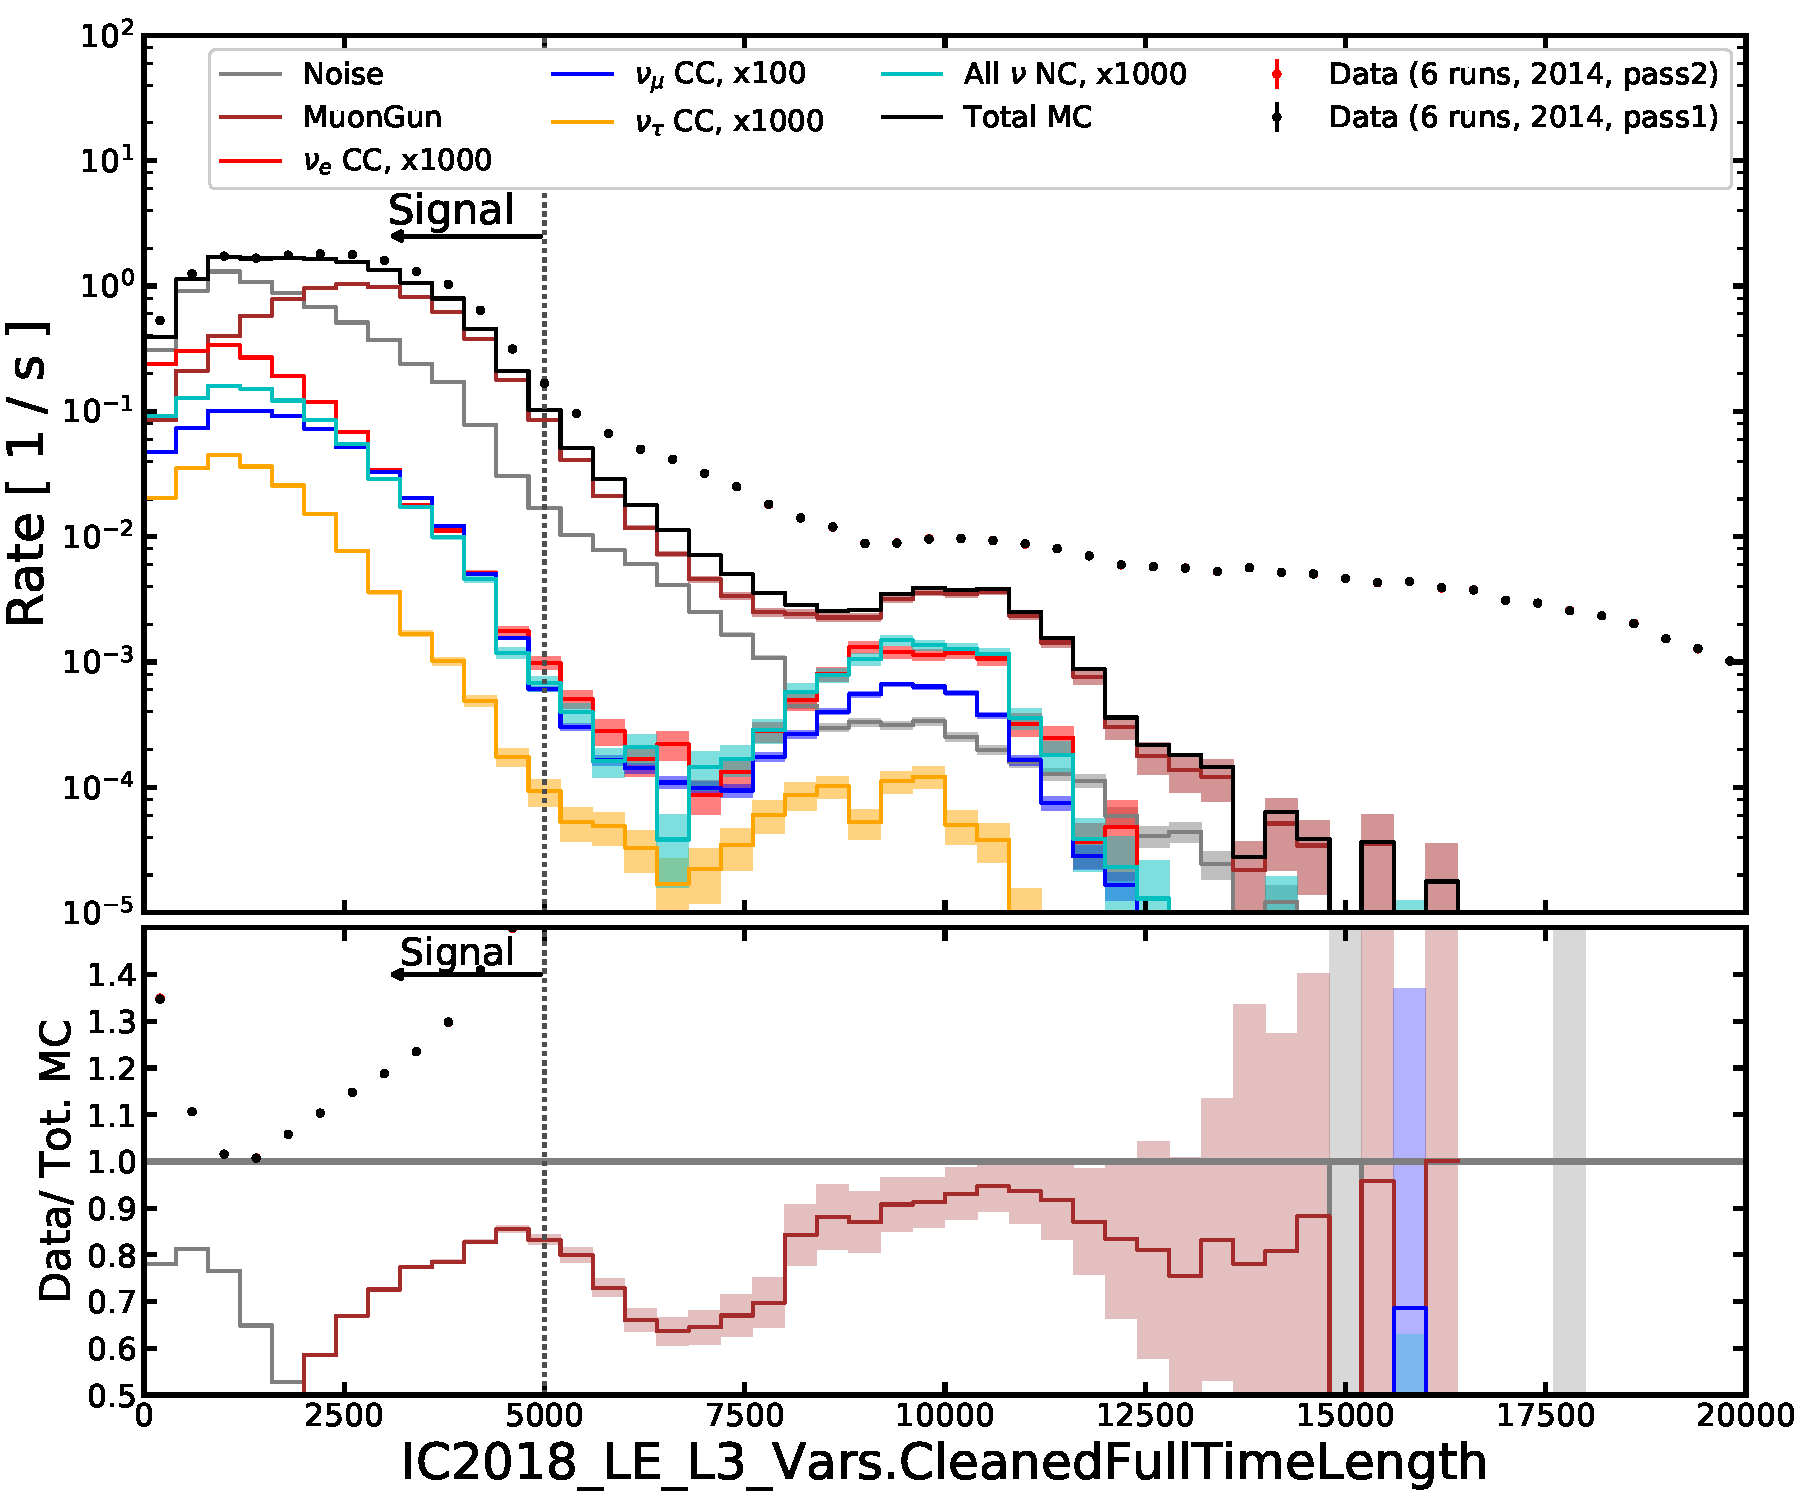
\includegraphics[width=7 cm]{figures/icecube/selection/IC2018_LE_L3_Vars_CleanedFullTimeLength.pdf}
%     \tikzsetnextfilename{l3_cleaned_full_time_length}%
\begin{tikzpicture}
    \pgfplotstableread{figures/icecube/selection/Level3/CleanedFullTimeLength_level3_data_mc_hists.csv}\table
    \begin{groupplot}[
        % xmin=0.0,xmax=25000.0,
        % this filter is applied to all x-coordinates in all plots!
        % Note that this filter would have to work on the *log* of the coordinates
        % if the x-axis was a log-axis (i.e. instead of scaling, you would shift).
        x filter/.expression={x*1e-3},
        xmin=0.0,xmax=25,
        xmajorgrids, ymajorgrids,
        width=0.45\linewidth,
        % The line below sets the position of the y-labels for all axes in
        % relative coordinates. Comment out to set positions automatically (which
        % may result in the "data/MC ratio" label being set a bit too far inside).
        ylabel style={at={(-0.15,0.5)}},
        group/.cd,
        group size=1 by 2,
        xticklabels at=edge bottom,
        vertical sep=10pt
        ]
    \nextgroupplot[
        height=0.35\linewidth,
        legend cell align={left},
        legend columns=4,
        legend to name=l3_vars_legend,
        legend style={
          at={(0.95,0.95)},
          anchor=north east,
        },
        ymode=log,
        % ymin=1e-05, ymax=1000.0,
        ymin=2e-5, ymax=5e2,
        ytick distance=1e1,
        ylabel={rate (Hz)},
        y filter/.expression={y < 1e-6 ? ln(1e-6) : ln(y)}
    ]
    % for some reason we called the column "muon", not "muons"...
    \ploterrorband[muon_color]{muon}{1}
    \addlegendentry{atm. muons}
    \ploterrorband[nue_color]{nue}{100}
    \addlegendentry{$\nu_e + \bar{\nu}_e$ x100}
    \ploterrorband[numu_color]{numu}{100}
    \addlegendentry{$\nu_\mu + \bar{\nu}_\mu$ x100}
    \ploterrorband[nutau_color]{nutau}{1000}
    \addlegendentry{$\nu_\tau + \bar{\nu}_\tau$ x1000}
    \ploterrorband[noise_color]{noise}{1}
    \addlegendentry{noise}
    \ploterrorband{total_mc}{1}
    \addlegendentry{total MC}

    \ploterrorbar{data}
    \addlegendentry{data (2014, 12 runs)}

    % draw cut
    % use "axis cs" to give coordinates in the data coordinate system!

    % \draw[thick,dashed] (axis cs:5000,1e-4) -- (axis cs:5000,100);
    % \draw[-stealth, very thick] (axis cs:5000,10)  -- node[anchor=south]{signal} (axis cs:1000,10);

    % since we scaled the coordnates to microseconds, we also need to use that for drawing
    \draw[thick,dashed] (axis cs:5,1e-6) -- (axis cs:5,100);
    \draw[-stealth, very thick] (axis cs:5,10)  -- node[anchor=south]{\footnotesize\sffamily signal} (axis cs:1,10);

    \nextgroupplot[
        height=0.2\linewidth,
        ymin=-0.1, ymax=2.85,
        ylabel=rate/total MC,
        xlabel={CleanedFullTimeLength ($\mu$s)}
    ]
   
    \ploterrorbar{data_mc_ratio}
    \plotratioerrorband[muon_color]{muon}{total_mc}
    \plotratioerrorband[nue_color]{nue}{total_mc}
    \plotratioerrorband[numu_color]{numu}{total_mc}
    \plotratioerrorband[nutau_color]{nutau}{total_mc}
    \plotratioerrorband[noise_color]{noise}{total_mc}
    
    \end{groupplot}
\end{tikzpicture}

%     \caption{Distribution of one of the variables used in the L3 offline filter, the time between the last hit and the first hit after noise cleaning. Histograms show the distributions in simulated data separated by particle and interaction type, data points with error bars show the distribution of real data. The bottom panel shows the ratio between data and simulation. Events falling on the "signal" side of the histogram are passed to the next filter level.}
%     \label{fig:l3-var-cleaned-full-time-length}
% \end{figure}

\begin{figure*}
    \centering
    \ref{l3_vars_legend}\par
    \tikzsetnextfilename{l3_cleaned_full_time_length}%
\begin{tikzpicture}
    \pgfplotstableread{figures/icecube/selection/Level3/CleanedFullTimeLength_level3_data_mc_hists.csv}\table
    \begin{groupplot}[
        % xmin=0.0,xmax=25000.0,
        % this filter is applied to all x-coordinates in all plots!
        % Note that this filter would have to work on the *log* of the coordinates
        % if the x-axis was a log-axis (i.e. instead of scaling, you would shift).
        x filter/.expression={x*1e-3},
        xmin=0.0,xmax=25,
        xmajorgrids, ymajorgrids,
        width=0.45\linewidth,
        % The line below sets the position of the y-labels for all axes in
        % relative coordinates. Comment out to set positions automatically (which
        % may result in the "data/MC ratio" label being set a bit too far inside).
        ylabel style={at={(-0.15,0.5)}},
        group/.cd,
        group size=1 by 2,
        xticklabels at=edge bottom,
        vertical sep=10pt
        ]
    \nextgroupplot[
        height=0.35\linewidth,
        legend cell align={left},
        legend columns=4,
        legend to name=l3_vars_legend,
        legend style={
          at={(0.95,0.95)},
          anchor=north east,
        },
        ymode=log,
        % ymin=1e-05, ymax=1000.0,
        ymin=2e-5, ymax=5e2,
        ytick distance=1e1,
        ylabel={rate (Hz)},
        y filter/.expression={y < 1e-6 ? ln(1e-6) : ln(y)}
    ]
    % for some reason we called the column "muon", not "muons"...
    \ploterrorband[muon_color]{muon}{1}
    \addlegendentry{atm. muons}
    \ploterrorband[nue_color]{nue}{100}
    \addlegendentry{$\nu_e + \bar{\nu}_e$ x100}
    \ploterrorband[numu_color]{numu}{100}
    \addlegendentry{$\nu_\mu + \bar{\nu}_\mu$ x100}
    \ploterrorband[nutau_color]{nutau}{1000}
    \addlegendentry{$\nu_\tau + \bar{\nu}_\tau$ x1000}
    \ploterrorband[noise_color]{noise}{1}
    \addlegendentry{noise}
    \ploterrorband{total_mc}{1}
    \addlegendentry{total MC}

    \ploterrorbar{data}
    \addlegendentry{data (2014, 12 runs)}

    % draw cut
    % use "axis cs" to give coordinates in the data coordinate system!

    % \draw[thick,dashed] (axis cs:5000,1e-4) -- (axis cs:5000,100);
    % \draw[-stealth, very thick] (axis cs:5000,10)  -- node[anchor=south]{signal} (axis cs:1000,10);

    % since we scaled the coordnates to microseconds, we also need to use that for drawing
    \draw[thick,dashed] (axis cs:5,1e-6) -- (axis cs:5,100);
    \draw[-stealth, very thick] (axis cs:5,10)  -- node[anchor=south]{\footnotesize\sffamily signal} (axis cs:1,10);

    \nextgroupplot[
        height=0.2\linewidth,
        ymin=-0.1, ymax=2.85,
        ylabel=rate/total MC,
        xlabel={CleanedFullTimeLength ($\mu$s)}
    ]
   
    \ploterrorbar{data_mc_ratio}
    \plotratioerrorband[muon_color]{muon}{total_mc}
    \plotratioerrorband[nue_color]{nue}{total_mc}
    \plotratioerrorband[numu_color]{numu}{total_mc}
    \plotratioerrorband[nutau_color]{nutau}{total_mc}
    \plotratioerrorband[noise_color]{noise}{total_mc}
    
    \end{groupplot}
\end{tikzpicture}

    \tikzsetnextfilename{l3_vertex_guess_z}%
\begin{tikzpicture}
    \pgfplotstableread{figures/icecube/selection/Level3/VertexGuessZ_level3_data_mc_hists.csv}\table
    \begin{groupplot}[
        xmin=-600,xmax=600,
        xmajorgrids, ymajorgrids,
        width=0.45\linewidth,
        % The line below sets the position of the y-labels for all axes in 
        % relative coordinates. Comment out to set positions automatically (which 
        % may result in the "data/MC ratio" label being set a bit too far inside).
        ylabel style={at={(-0.15,0.5)}},
        group/.cd,
        group size=1 by 2,
        xticklabels at=edge bottom,
        vertical sep=10pt
        ]
    \nextgroupplot[
        height=0.35\linewidth,
        legend cell align={left},
        legend columns=1,
        legend to name=l3_vars_legend_vertex_guess,
        ymode=log,
        ymin=2e-5, ymax=5e2,
        ytick distance=1e1,
        ylabel={rate (Hz)},
        y filter/.expression={y < 1e-6 ? ln(1e-6) : ln(y)}
    ]
    % for some reason we called the column "muon", not "muons"...
    \ploterrorband[muon_color]{muon}{1}
    \addlegendentry{atm. muons}
    \ploterrorband[nue_color]{nue}{100}
    \addlegendentry{$\nu_e + \bar{\nu}_e$ x100}
    \ploterrorband[numu_color]{numu}{100}
    \addlegendentry{$\nu_\mu + \bar{\nu}_\mu$ x100}
    \ploterrorband[nutau_color]{nutau}{1000}
    \addlegendentry{$\nu_\tau + \bar{\nu}_\tau$ x1000}
    \ploterrorband[noise_color]{noise}{1}
    \addlegendentry{noise}
    \ploterrorband{total_mc}{1}

    \ploterrorbar{data}
    \addlegendentry{data (2014, 12 runs)}

    \draw[thick,dashed] (axis cs:-120,1e-6) -- (axis cs:-120,100);
    \draw[-stealth, very thick] (axis cs:-120,5)  -- node[anchor=south]{\footnotesize\sffamily signal} (axis cs:-400,5);

    \nextgroupplot[
        height=0.2\linewidth,
        ymin=0.5, ymax=4,
        ylabel={data/MC ratio},
        xlabel={first HLC z-position}
    ]
    \ploterrorband{data_mc_ratio}{1}
    \end{groupplot}
\end{tikzpicture}

    
    \caption{Distribution of one of the variables used in the L3 offline filter, the time between the last hit and the first hit after noise cleaning (left) and the z-position of the first HLC hit (right). Histograms show the distributions in simulated data separated by particle and interaction type, data points with error bars show the distribution of real data. The bottom panel shows the ratio between data and simulation. Events falling on the "signal" side of the histogram are passed to the next filter level.}
    \label{fig:l3-cut-vars}
\end{figure*}

\subsubsection{Level 4}
\label{sec:level4-selection}
In the next level, L4, more advanced selections based on the output of Boosted Decision Trees (BDTs) are applied, with a separately trained BDT for noise and muon rejection, respectively. The output of each BDT is a probability score between zero (background-like) and one (signal-like).  The inputs into the BDT aimed at noise rejection consist of hit counts in cleaned hit series and variables that characterize the geometric and temporal spread of the observed hits, such as the full width half maximum (FWHM) of the hit times. The BDT is trained using simulated pure noise and neutrino events. Events are passing the L4 noise cut if the BDT score is above 0.7, which reduces the number of pure noise events by two orders of magnitude from 36.6~mHz to approximately 0.3~mHz. The BDT that is used to reject atmospheric muons also takes simple variables as its input that consist mostly of different veto hit counts and variables that characterize the distribution of z-coordinates of the observed hits as well as their radial distance with respect to the center of the DeepCore fiducial volume. In contrast to the noise BDT, however, the muon BDT is trained using real data and simulated neutrino events, with the goal of rejecting data events. This is possible because the data sample consists to 99\% of atmospheric muons at this stage of the event selection. Events pass the L4 muon cut if the output score of the muon BDT is greater than 0.65, removing 94\% of all muon events while keeping 87\% of all neutrinos. The distributions of the output scores of both BDTs are shown in figure~\ref{fig:l4-bdt-output}.
\begin{figure*}
    \centering
    %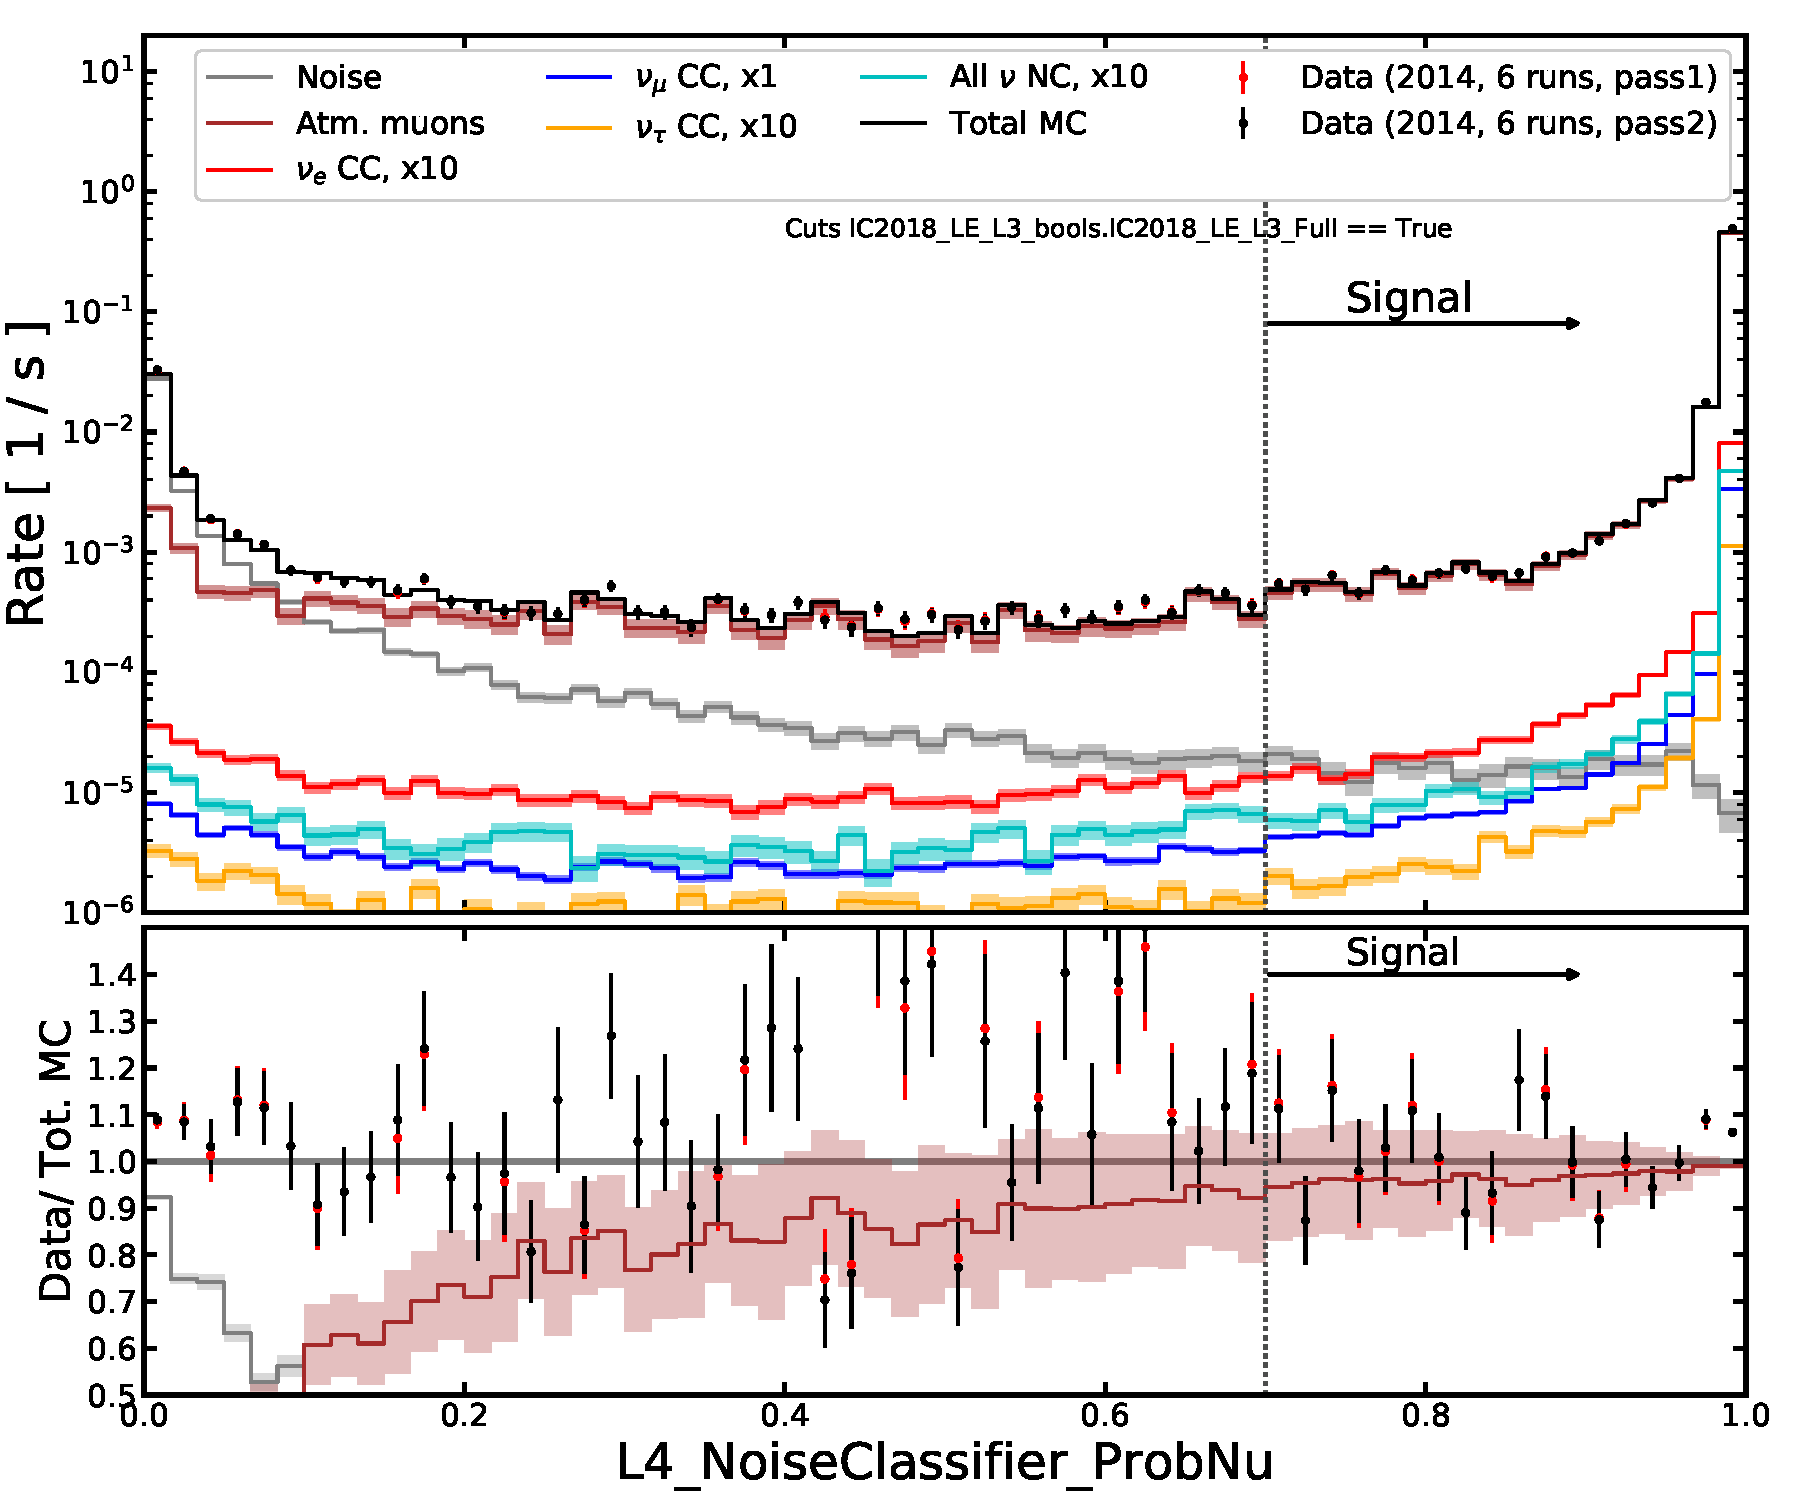
\includegraphics[width=7 cm]{figures/icecube/selection/L4_noiseBDT_L4_NoiseClassifier_ProbNu.pdf}
    %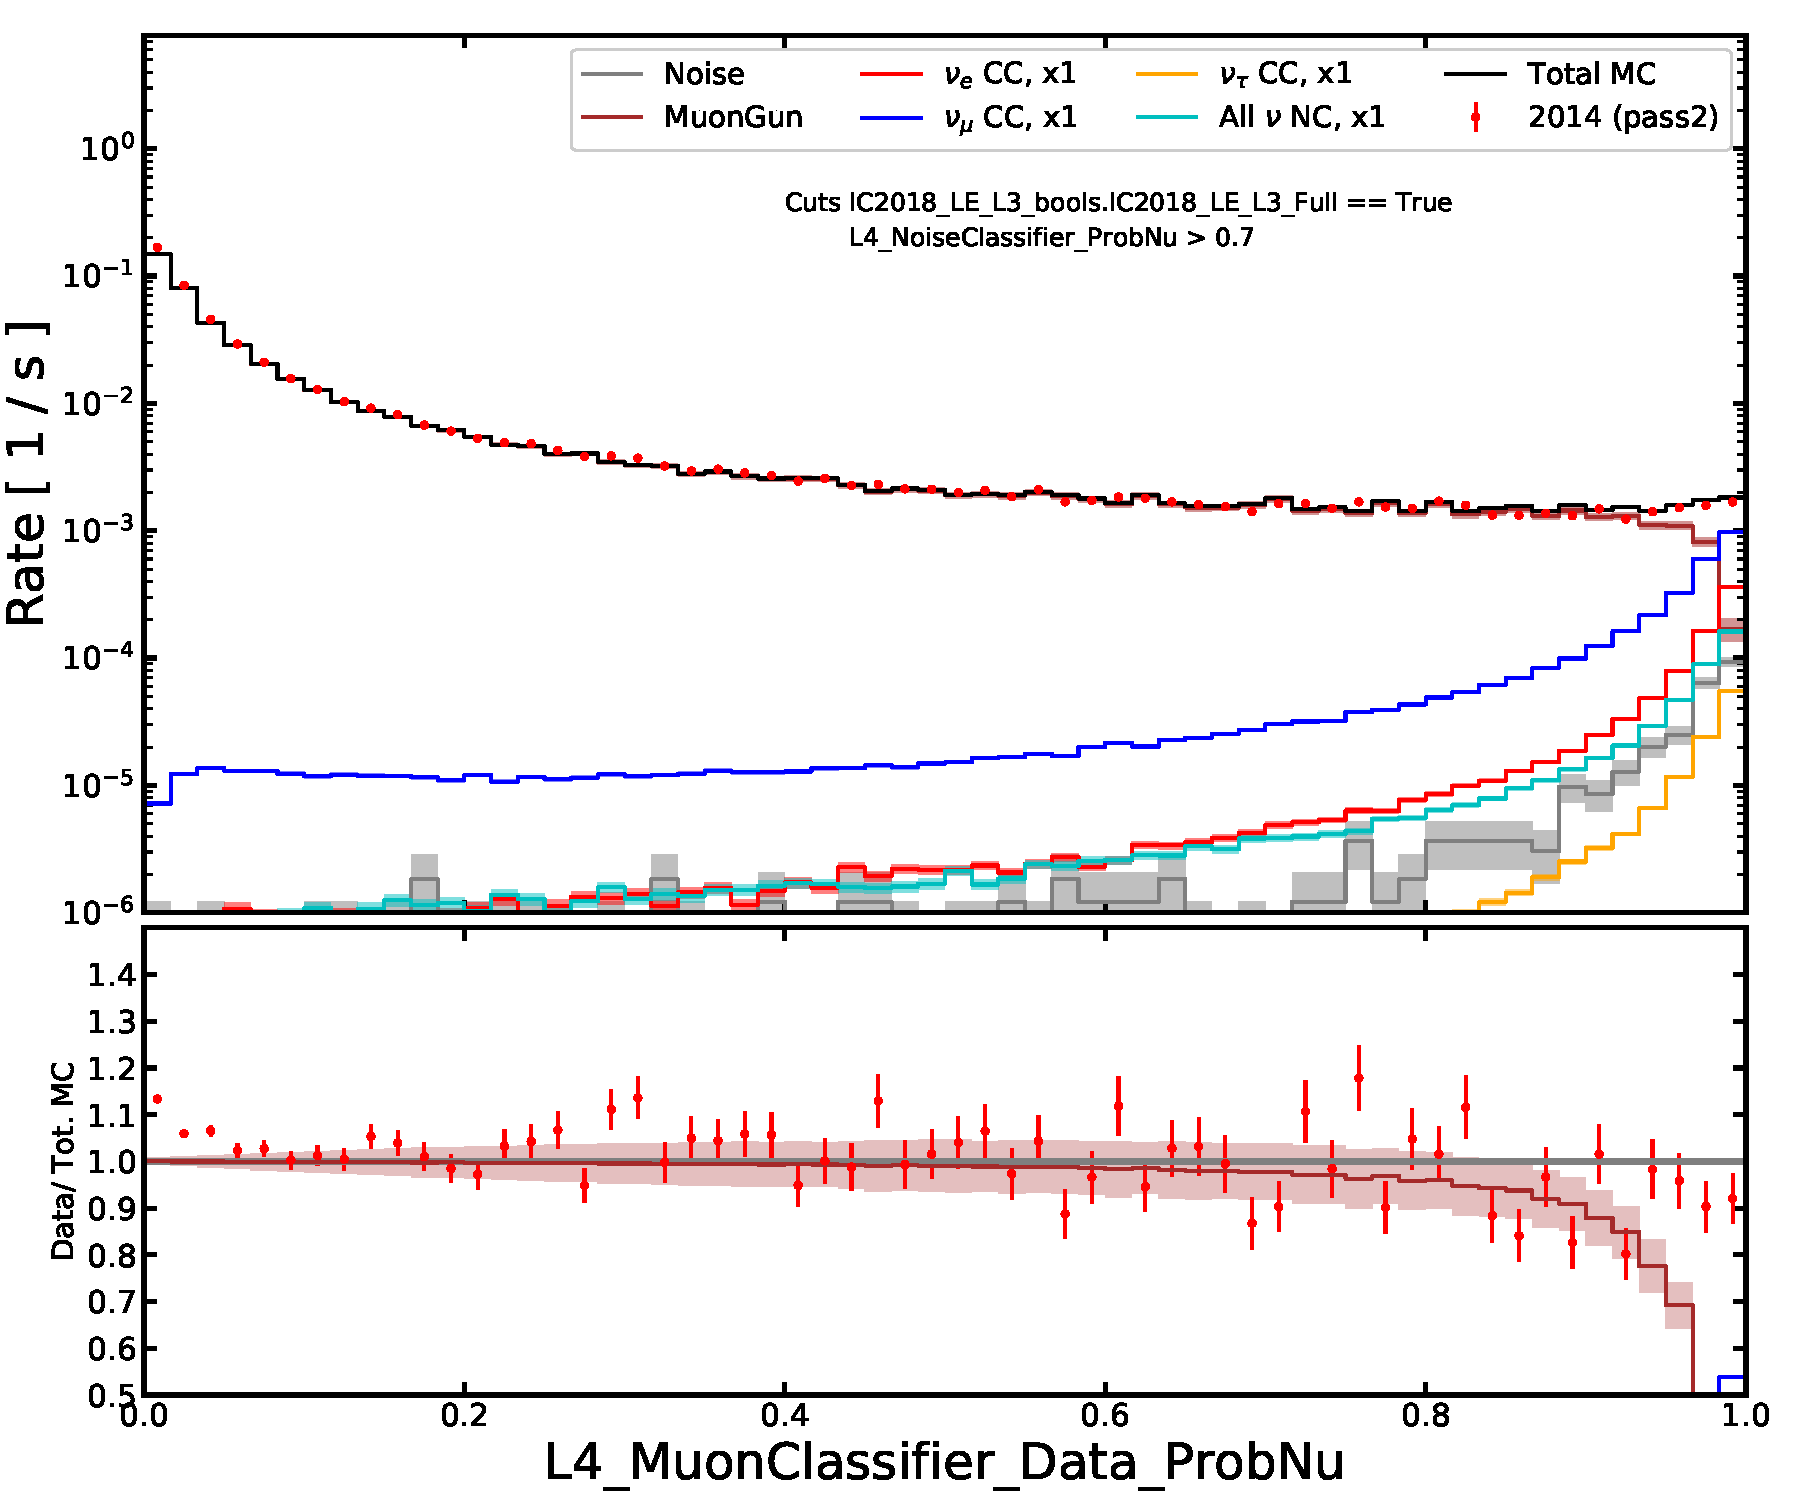
\includegraphics[width=7 cm]{figures/icecube/selection/L4_muon_L4_MuonClassifier_Data_ProbNu.pdf}
    \ref{l4_bdt_hist_legend}\hfill
    \tikzsetnextfilename{l4_noise_classifier_probnu}%
\begin{tikzpicture}
    \pgfplotstableread{figures/icecube/selection/Level4/L4_NoiseClassifier_ProbNu_level4_data_mc_hists.csv}\table
    \begin{groupplot}[
        xmin=0.0,xmax=1.0,
        xmajorgrids, ymajorgrids,
        width=0.45\linewidth,
        ylabel style={at={(-0.15,0.5)}},
        group/.cd,
        group size=1 by 2,
        xticklabels at=edge bottom,
        vertical sep=10pt,
        %every axis y label style={xshift=0.5 cm}
        ]
    \nextgroupplot[
        height=0.35\linewidth,
        legend cell align={left},
        % legend columns=-1,
        legend to name=l4_bdt_hist_legend,
        legend columns=-1,
        ymode=log,
        ymin=1e-07, ymax=1.0,
        ylabel={rate (Hz)},
        ytick distance=1e1
    ]
    \ploterrorband[muon_color]{muons}{1}
    \addlegendentry{atm. muons}
    \ploterrorband[nu_color]{nu}{1}
    \addlegendentry{atm. $\nu$}
    % \ploterrorband[nue_color]{nue}{1}
    % \addlegendentry{$\nu_e + \bar{\nu}_e$}
    % \ploterrorband[numu_color]{numu}{1}
    % \addlegendentry{$\nu_\mu + \bar{\nu}_\mu$}
    % \ploterrorband[nutau_color]{nutau}{1}
    % \addlegendentry{$\nu_\tau + \bar{\nu}_\tau$}
    \ploterrorband[noise_color]{noise}{1}
    \addlegendentry{noise}
    \ploterrorband{total_mc}{1}
    \addlegendentry{total MC}
    \ploterrorbar{data}
    \addlegendentry{season 2014
    (12 runs)}

    % draw cut
    \draw[thick,dashed] (axis cs:0.7,1e-7) -- (axis cs:0.7,10);
    \draw[-stealth, very thick] (axis cs:0.7,2e-2)  -- node[anchor=south]{\footnotesize\sffamily signal} (axis cs:0.9,2e-2);

    \nextgroupplot[
        height=0.2\linewidth,
        ymin=-0.1, ymax=1.8,
        ylabel=rate/total MC,
        xlabel={L4 NoiseClassifier ProbNu}
    ]

    \ploterrorbar{data_mc_ratio}
    \plotratioerrorband[muon_color]{muons}{total_mc}
    \plotratioerrorband[nu_color]{nu}{total_mc}
    % \plotratioerrorband[nue_color]{nue}{total_mc}
    % \plotratioerrorband[numu_color]{numu}{total_mc}
    % \plotratioerrorband[nutau_color]{nutau}{total_mc}
    \plotratioerrorband[noise_color]{noise}{total_mc}
    \end{groupplot}
\end{tikzpicture}

    \tikzsetnextfilename{l4_muon_classifier_probnu}%
\begin{tikzpicture}
    \pgfplotstableread{figures/icecube/selection/Level4/L4_MuonClassifier_Data_ProbNu_level4_data_mc_hists.csv}\table
    \begin{groupplot}[
        xmin=0.0,xmax=1.0,
        xmajorgrids, ymajorgrids,
        width=0.45\linewidth,
        ylabel style={at={(-0.15,0.5)}},
        group/.cd,
        group size=1 by 2,
        xticklabels at=edge bottom,
        vertical sep=10pt
        ]
    \nextgroupplot[
        height=0.35\linewidth,
        legend cell align={left},
        legend columns=2,
        ymode=log,
        ymin=1e-07, ymax=1.0,
        ylabel={rate (Hz)},
        ytick distance=1e1
    ]
    \ploterrorband[muon_color]{muons}{1}
    % \addlegendentry{atm. muons}
    \ploterrorband[nu_color]{nu}{1}
    % \addlegendentry{atm. $\nu$}
    % \ploterrorband[nue_color]{nue}{1}
    % % \addlegendentry{$\nu_e + \bar{\nu}_e$ x10}
    % \ploterrorband[numu_color]{numu}{1}
    % % \addlegendentry{$\nu_\mu + \bar{\nu}_\mu$ x10}
    % \ploterrorband[nutau_color]{nutau}{1}
    % % \addlegendentry{$\nu_\tau + \bar{\nu}_\tau$ x100}
    \ploterrorband[noise_color]{noise}{1}
    % \addlegendentry{noise}
    \ploterrorband{total_mc}{1}
    % \addlegendentry{total MC}

    \addplot[
        mark=*,
        mark options={scale=0.5, fill=black},
        black,
        only marks,
        error bars/.cd,
        x dir=none,
        y dir=both,
        y explicit,
    ] table [x=bin_midpoints, y=data, y error=data__err]  from \table;
    % \addlegendentry{season 2014 (12 runs)}

    % draw cut
    \draw[thick,dashed] (axis cs:0.65,1e-7) -- (axis cs:0.65,10);
    \draw[-stealth, very thick] (axis cs:0.65,2e-2)  -- node[anchor=south]{\footnotesize\sffamily signal} (axis cs:0.85,2e-2);

    \nextgroupplot[
        height=0.2\linewidth,
        ymin=-0.1, ymax=1.8,
        ylabel=rate/total MC,
        xlabel={L4 MuonClassifier Data ProbNu}
    ]

    \ploterrorbar{data_mc_ratio}
    \plotratioerrorband[muon_color]{muons}{total_mc}
    \plotratioerrorband[nu_color]{nu}{total_mc}
    % \plotratioerrorband[nue_color]{nue}{total_mc}
    % \plotratioerrorband[numu_color]{numu}{total_mc}
    % \plotratioerrorband[nutau_color]{nutau}{total_mc}
    \plotratioerrorband[noise_color]{noise}{total_mc}

    \end{groupplot}
\end{tikzpicture}

    
    \caption{Distribution scores for the noise (left) and muon (right) BDT. The distributions of the muon classifier are shown for events where the score of the noise BDT is greater than 0.7.}
    \label{fig:l4-bdt-output}
\end{figure*}

\subsubsection{Level 5}
The final filter that is applied before the event reconstruction step is L5. This filter searches specifically for hits occurring in un-instrumented \emph{corridors} within the IceCube array through which an atmospheric muon can sneak into the DeepCore volume while evading previous veto cuts. In addition, events with more than seven hits in the outermost strings of the IceCube array or that have a down-going pattern of hits in the uppermost region of the detector are vetoed to remove events containing atmospheric muons entering the detector coincidentally with neutrinos. The distribution for one of the corridor variables and one of the muon rejection variables are shown in figure~\ref{fig:l5-vars}. Table~\ref{tab:l5_summary} shows the rates of each event type expected at each level of the selection up to L5 together with the efficiency of the filter at the final level.
\begin{figure*}
    \centering
    % 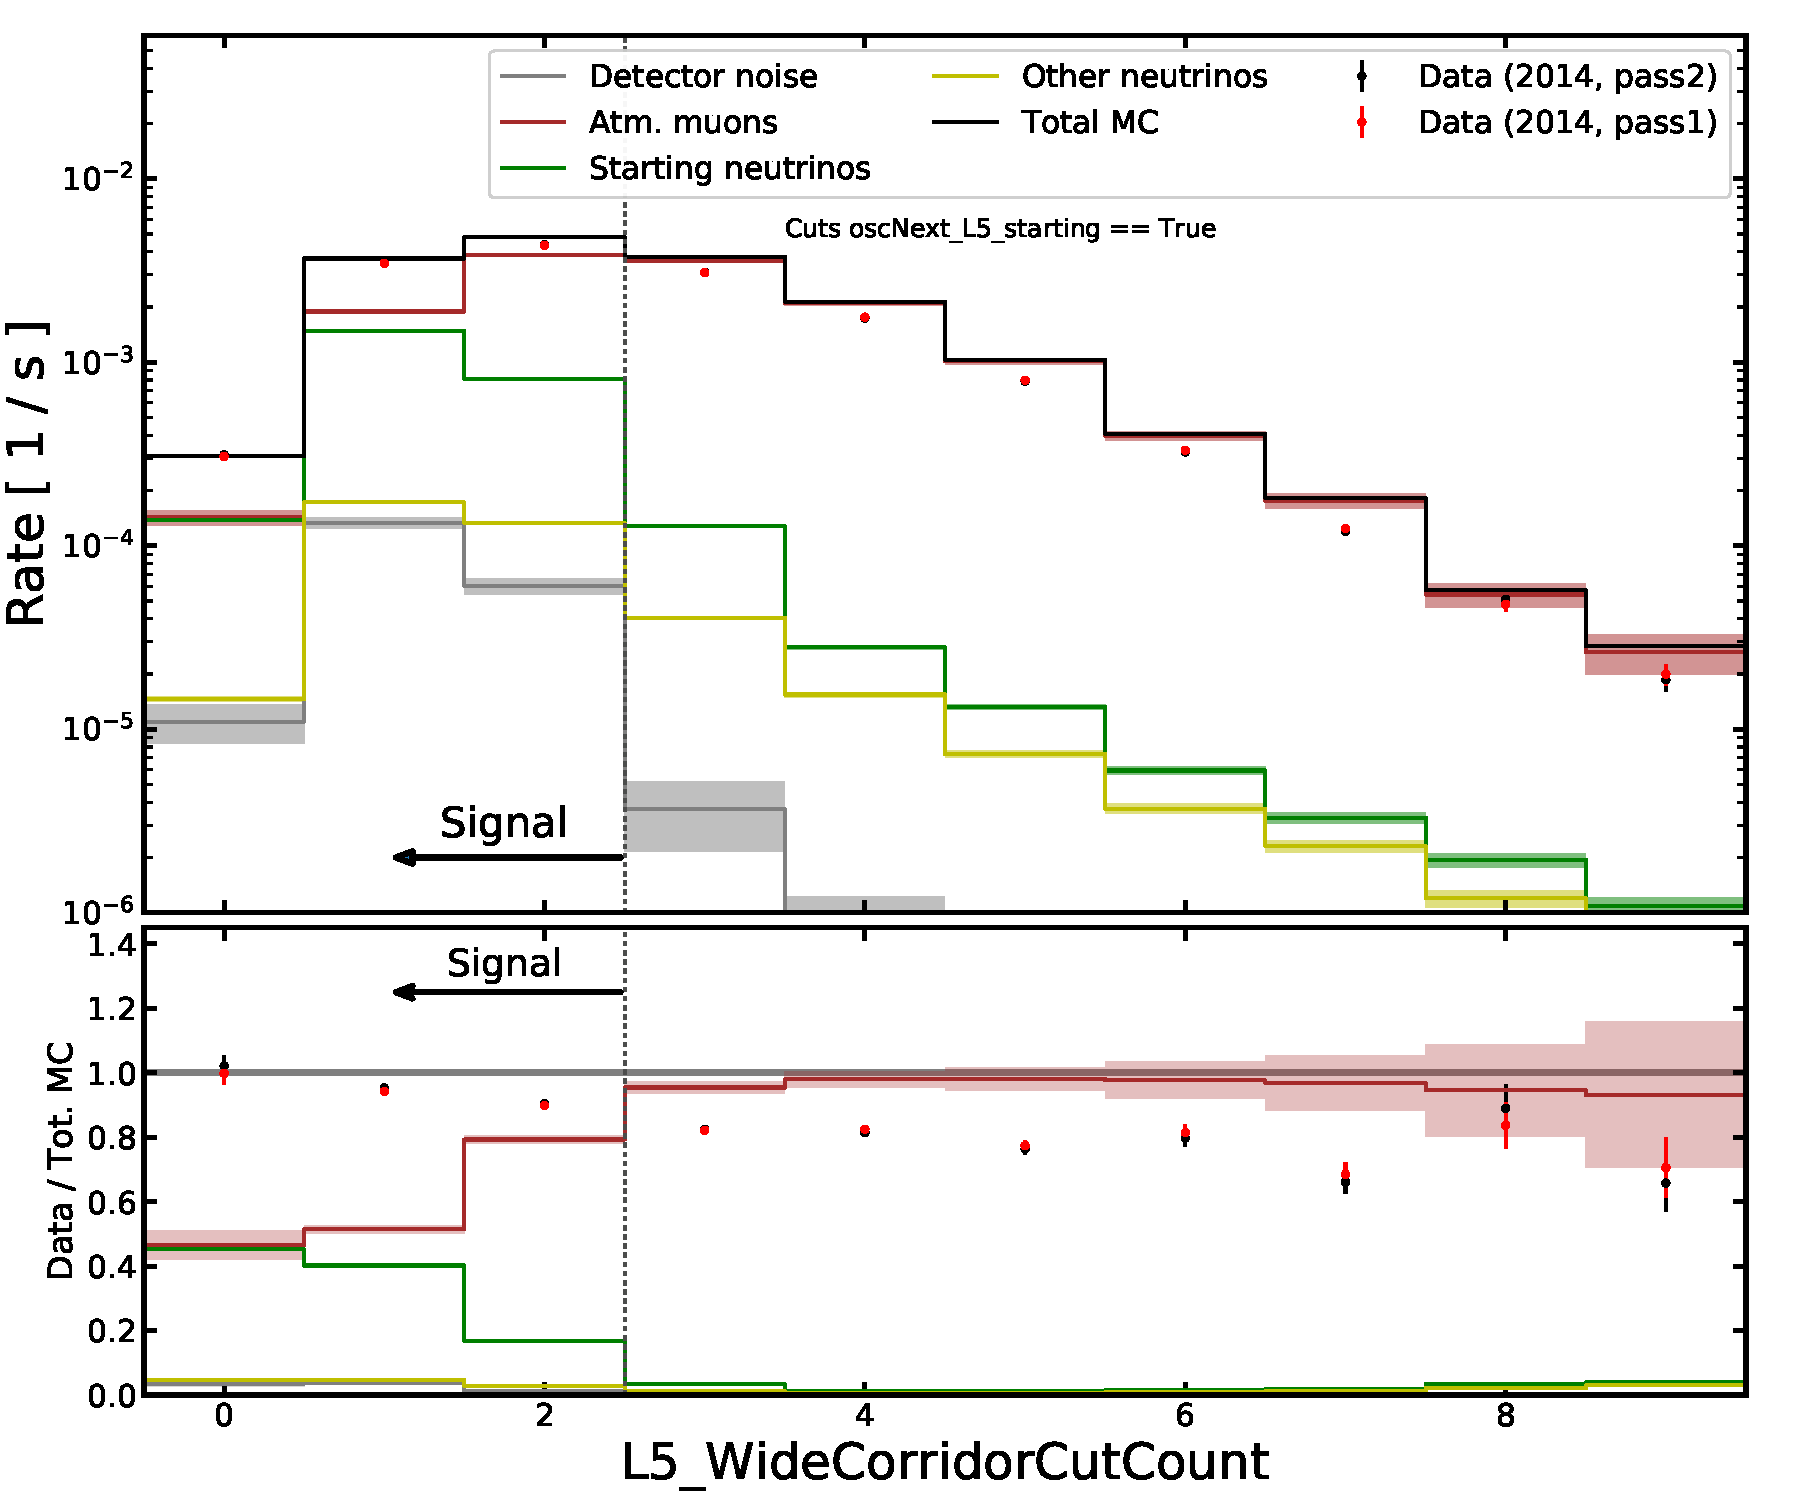
\includegraphics[width=7 cm]{figures/icecube/selection/L5_contained_L5_WideCorridorCutCount.pdf}
    % 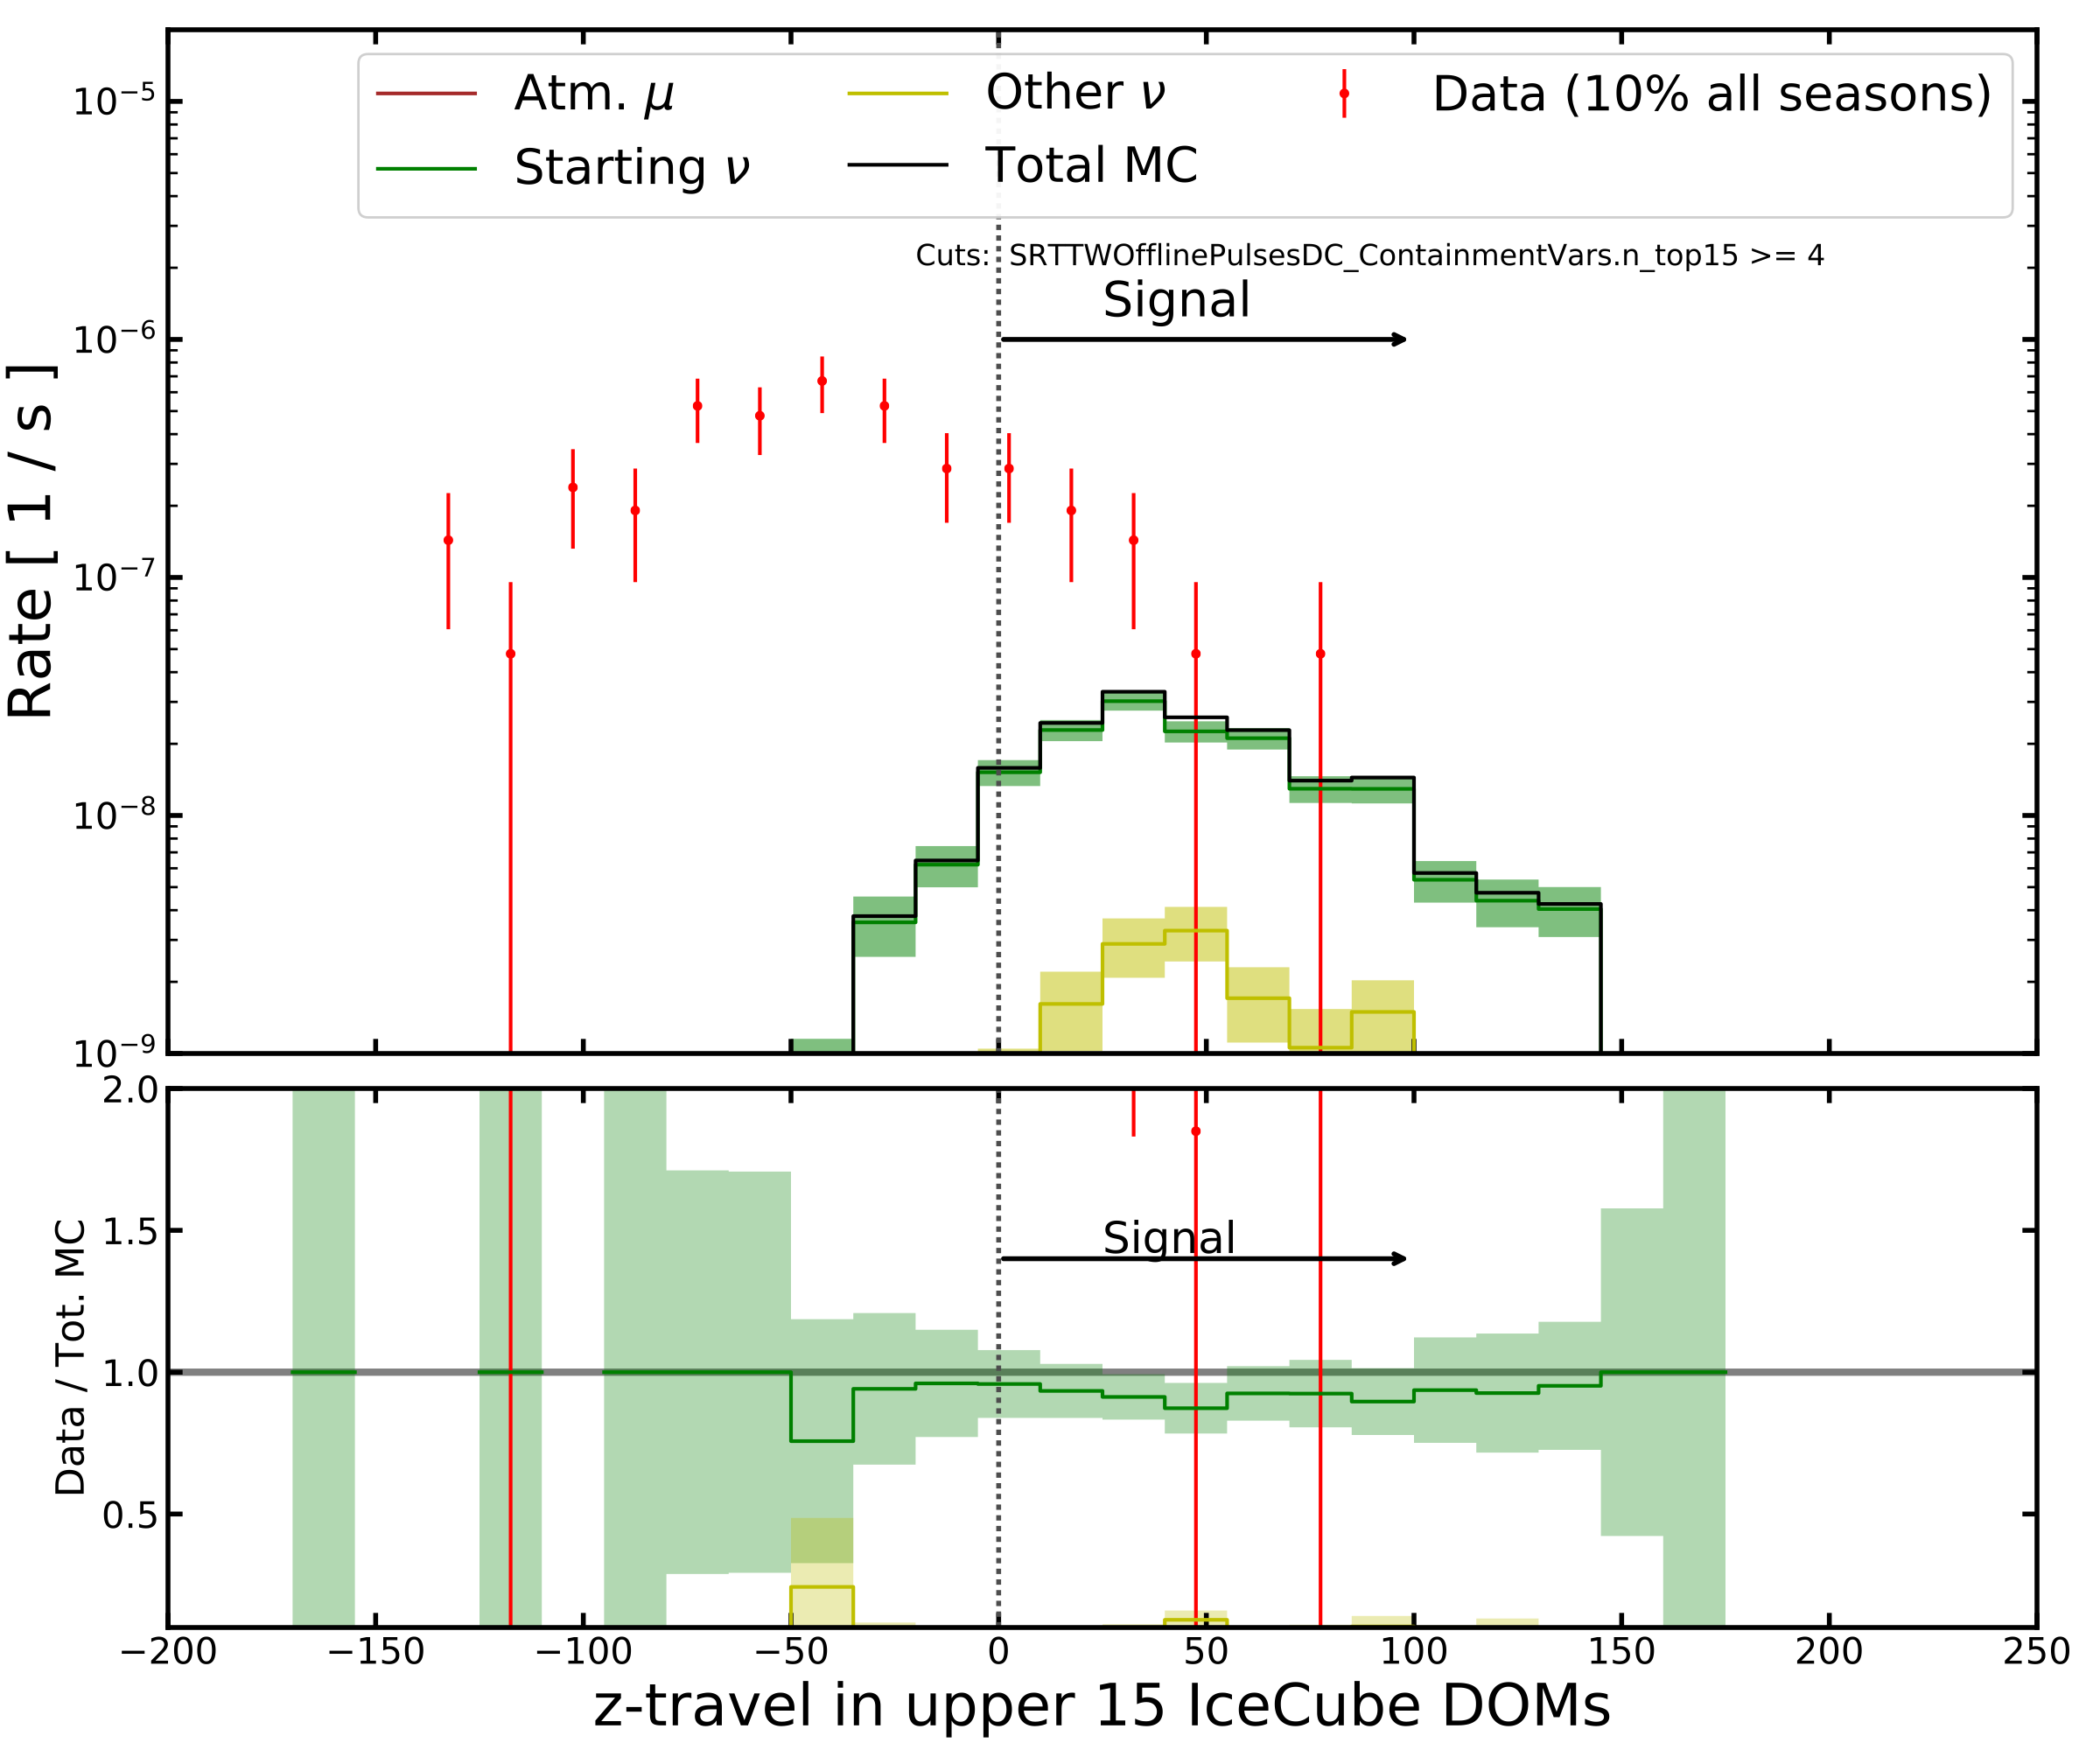
\includegraphics[width=7 cm]{figures/icecube/selection/SRTTWOfflinePulsesDC_ContainmentVars.z_travel_top15.png}
    \ref{l5_corridor_vars_legend}
    \tikzsetnextfilename{l5_corridor_cut_count}%
\begin{tikzpicture}
    \pgfplotstableread{figures/icecube/selection/Level5/L5_WideCorridorCutCount_level5_data_mc_hists.csv}\table
    \begin{groupplot}[
        xmin=0,xmax=15,
        xmajorgrids, ymajorgrids,
        width=0.45\linewidth,
        ylabel style={at={(-0.15,0.5)}},
        %scale only axis=true,
        group/.cd,
        group size=1 by 2,
        xticklabels at=edge bottom,
        vertical sep=10pt
        ]
    \nextgroupplot[
        height=0.3\linewidth,
        legend cell align={left},
        legend columns=4,
        legend to name=l5_corridor_vars_legend,
        ymode=log,
        ymin=5e-06, ymax=0.2,
        ytick distance=1e1,
        ylabel={rate (Hz)},
        y filter/.expression={y < 1e-7 ? ln(1e-8) : ln(y)}
    ]

    \ploterrorband[muon_color]{muons}{1}
    \addlegendentry{atm. muons}
    \ploterrorband[nue_color]{nue}{1}
    \addlegendentry{$\nu_e + \bar{\nu}_e$}
    \ploterrorband[numu_color]{numu}{1}
    \addlegendentry{$\nu_\mu + \bar{\nu}_\mu$}
    \ploterrorband[nutau_color]{nutau}{1}
    \addlegendentry{$\nu_\tau + \bar{\nu}_\tau$}
    \ploterrorband[noise_color]{noise}{1}
    \addlegendentry{noise}
    \ploterrorband{total_mc}{1}
    \addlegendentry{total MC}
    \addplot[
        mark=*,
        mark options={scale=0.5, fill=black},
        black,
        only marks,
        error bars/.cd,
        x dir=none,
        y dir=both,
        y explicit
    ] table [x=bin_midpoints, y=data, y error=data__err]  from \table;
    \addlegendentry{season 2014
    (12 runs)}

    % draw cut
    \draw[thick,dashed] (axis cs:2,1e-6) -- (axis cs:2,1e-1);
    \draw[stealth-, very thick] (axis cs:2,2e-2)  -- node[anchor=south]{\footnotesize\sffamily cut} (axis cs:5,2e-2);

    \nextgroupplot[
        height=0.2\linewidth,
        ymin=0, ymax=4,
        ylabel={data/MC ratio},
        xlabel={Number of hits in corridor\strut }
    ]

    \ploterrorband{data_mc_ratio}{1}
    \end{groupplot}
\end{tikzpicture}

    \tikzsetnextfilename{l5_corridor_angle_total_cos_diff}%
\begin{tikzpicture}
    \pgfplotstableread{figures/icecube/selection/Level5/L5_WideCorridorCutTrack_L5_SPEFit11_angles_total_cos_diff_level5_data_mc_hists.csv}\table
    \begin{groupplot}[
        xmin=-1.1,xmax=1.0,
        xmajorgrids, ymajorgrids,
        width=0.45\linewidth,
        ylabel style={at={(-0.15,0.5)}},
        %scale only axis=true,
        group/.cd,
        group size=1 by 2,
        xticklabels at=edge bottom,
        vertical sep=10pt
        ]
    \nextgroupplot[
        height=0.35\linewidth,
        legend cell align={left},
        legend columns=2,
        legend to name=l5_corridor_anglediff_legend,
        ymode=log,
        ymin=5e-06, ymax=2e-2,
        ytick distance=1e1,
        ylabel={rate (Hz)},
        y filter/.expression={y < 1e-7 ? ln(1e-7) : ln(y)}
    ]
    \ploterrorband[muon_color]{muons}{1}
    \addlegendentry{atm. muons}
    \ploterrorband[nue_color]{nue}{1}
    \addlegendentry{$\nu_e + \bar{\nu}_e$}
    \ploterrorband[numu_color]{numu}{1}
    \addlegendentry{$\nu_\mu + \bar{\nu}_\mu$}
    \ploterrorband[nutau_color]{nutau}{1}
    \addlegendentry{$\nu_\tau + \bar{\nu}_\tau$}
    \ploterrorband[noise_color]{noise}{1}
    \addlegendentry{noise}
    \ploterrorband{total_mc}{1}
    \addlegendentry{total MC}
    
    \addplot[
        mark=*,
        mark options={scale=0.5, fill=black},
        black,
        only marks,
        error bars/.cd,
        x dir=none,
        y dir=both,
        y explicit
    ] table [x=bin_midpoints, y=data, y error=data__err]  from \table;
    \addlegendentry{season 2014
    (12 runs)}

    % draw cut
    \draw[thick,dashed] (axis cs:0.7,1e-6) -- (axis cs:0.7,1e-2);
    \draw[-stealth, very thick] (axis cs:0.7,2e-3)  -- node[anchor=south]{\footnotesize\sffamily signal} (axis cs:0.2,2e-3);
    
    \nextgroupplot[
        height=0.2\linewidth,
        ymin=0, ymax=2,
        ylabel={data/MC ratio},
        xlabel={Cosine of angle difference to corridor\strut}
    ]
    \ploterrorband{data_mc_ratio}{1}

    \end{groupplot}
\end{tikzpicture}

    \caption{Distributions for one of the L5 corridor cut variables.}
    \label{fig:l5-vars}
\end{figure*}

\begin{table}
\begin{tabular}{lrrrrr}
Event type  & DC filter   & L3   & L4   & L5   & Eff. (\%) \\
\toprule
Atm. $\mu$         & 7273 & 505  & 28.1 & 0.93 & 0.012          \\
Pure noise         & 6621 & 36.6 & 0.28 & 0.07 & 0.001          \\
Atm. $\nu_e$ CC    & 1.61 & 0.95 & 0.84 & 0.48 & 29.8           \\
Atm. $\nu_\mu$ CC  & 6.16 & 3.77 & 3.11 & 1.39 & 22.5           \\
Atm. $\nu_\tau$ CC & 0.19 & 0.13 & 0.12 & 0.07 & 36.8           \\
Atm. $\nu$ NC      & 0.86 & 0.53 & 0.46 & 0.23 & 26.7  \\
\end{tabular}
\caption{Summary of the rates (in mHz) obtained after each level of selection. Neutrinos are weighted to an atmospheric spectrum with oscillations included.}
\label{tab:l5_summary}
\end{table}

\subsection{Event Reconstruction}
\label{sec:event-reconstruction}

After the L5 selection, the rate of muons is reduced enough so that the majority of the total sample is expected to consist of atmospheric neutrinos, and it is at this point that the event reconstruction and signature classification are run. For the measurement presented in this thesis, three reconstructed quantities are required: The zenith angle, the energy, and a proxy score determining the flavor of a neutrino. As described in Section \ref{sec:particle-signatures}, all neutrino events in DeepCore can be effectively approximated as a cascade ($\nu_e$ CC events, all NC events and 83\% of $\nu_\tau$ CC events) or a combination of a cascade at the neutrino interaction point with an outgoing muon track ($\nu_\mu$ CC events and 17\% of $\nu_\tau$ CC events). The zenith angle can be most accurately reconstructed for track-like events due to their elongated, highly directional signature. For cascades, the reconstruction of the direction is more difficult because of their most compact and diffuse light distribution. The energy of a neutrino event is reconstructed by comparing the expected light output of a combined track and cascade hypothesis with the observed hits. Finally, the flavor proxy is calculated using variables that characterize the elongation of the observed hit signature and the goodness of fit of a combined track and cascade hypothesis compared to that of a cascade-only hypothesis. The resulting score allows the separation of muon neutrino interactions from other interactions, which is ideally suitable to observe the muon neutrino disappearance oscillation channel.

\subsubsection{Zenith angle reconstruction}
\label{sec:santa}
The zenith angle is reconstructed using the Single-string Antares-inspired Analysis (\textsc{santa})\sidecite{Garza2014Measurement}. It is an older algorithm aimed at reconstructing the direction of muon tracks that was originally developed for use in the ANTARES neutrino telescope~\sidecite{Aguilar:2011zz}. It has since been refurbished and improved in IceCube, as described in detail in~\sidecite{lowen-reco-paper}.

The reconstructed pulse series in every DOM is summarized by the time of the first pulse and the sum of charges of all pulses. This time and charge are the only information used by the reconstruction and are referred to as a \emph{hit} in the following. The first step of the reconstruction algorithm is a cleaning routine that removes hits produced
by photons that have been scattered many times as they traveled
through the ice, leaving only hits from photons that have traveled in approximately straight lines based on the time difference between hits on the same string.
%The algorithm is a simplification from an earlier implementation described in \cite{Garza2014Measurement}.
It calculates the signal speed between hits on the same string, and removes a hit if this velocity is below the speed of light in ice. This is a simplification of the algorithm described in \cite{Garza2014Measurement}, where the effective signal velocity was updated during the selection process. The selection is run separately for each string, and if fewer than three hits remain on a string, all hits on the string are discarded. In total, it is necessary for at least five hits to remain in an event in order to run the directional reconstruction. If only hits on one string remain after the selection, the event is referred to as a \emph{single-string} event, otherwise it is a \emph{multi-string} event. The reconstruction is generally more accurate for multi-string events, because the spacing between strings provides a long lever arm to constrain the direction of a track. In addition, the azimuth angle of the track can only be reconstructed for \emph{multi-string} events due to the rotational symmetry of a single string.

\begin{figure*}
    \centering
    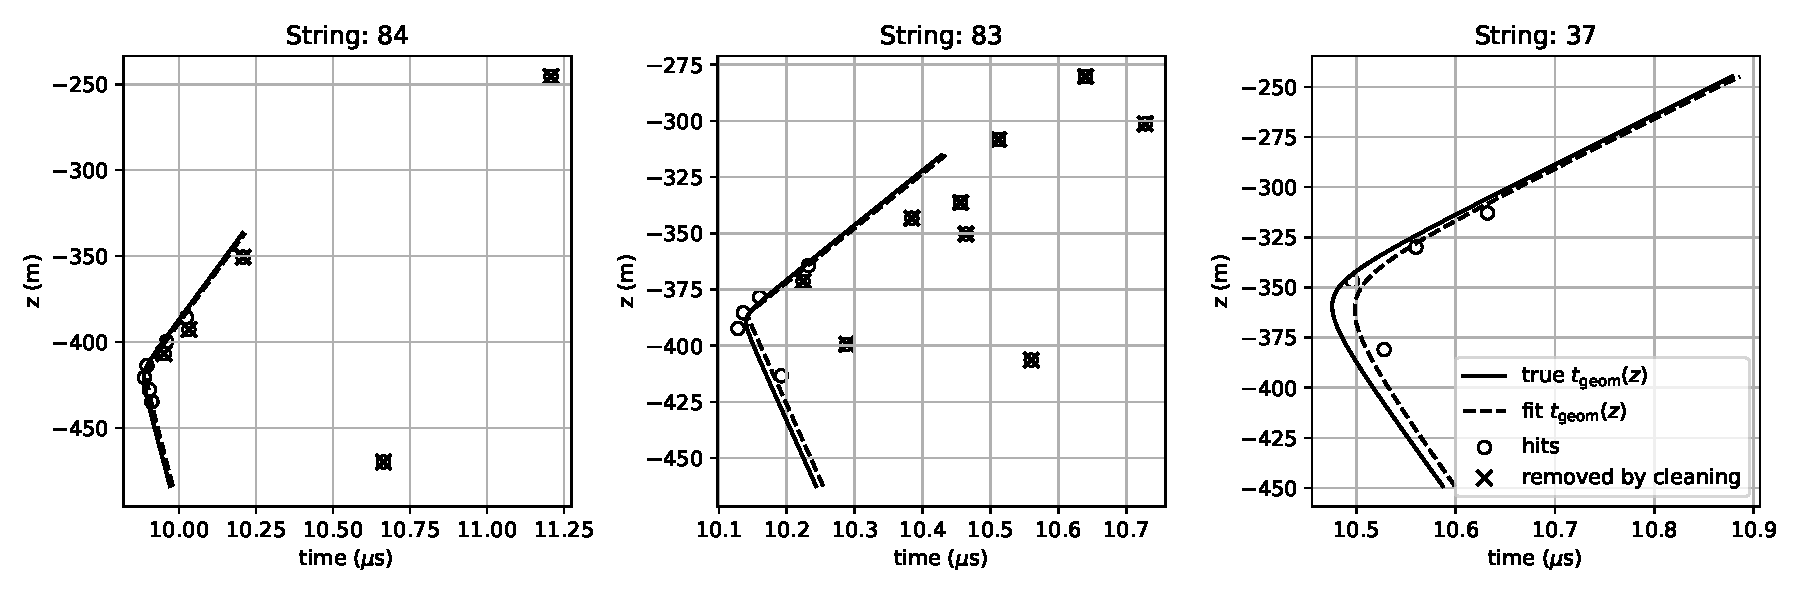
\includegraphics[width=\linewidth]{figures/icecube/reconstruction/santa/multi_string_example_with_cleaning_id_12607962.pdf}
    \caption{Example of a \numucc event reconstructed with \textsc{santa} with hits on several strings. Strings 84, 83 and 37 are spaced $\sim80\,\mathrm{m}$ apart from each other and form a highly obtuse triangle.}
    \label{fig:santa-multi-string-example}
\end{figure*}

The directional reconstruction itself is a regression the minimizes a modified $\chi^2$ loss with respect to the observed and predicted observation time with an additional regularization term involving the observed charge. Given a set of parameters characterizing the track, $\vec{\theta}$, the loss is defined as
\begin{equation}
L(\vec{\theta})=\sum_{i=1}^{N}\phi(r^2_i(\vec{\theta}))
+
\frac{1}{\bar{q}}\sum_{i=1}^{N}\tilde{q}_i \frac{d_{\gamma,i}}{d_0}\,.\label{eq:chi-square-mod-loss}
\end{equation}
where $\bar{q}$ is the average of $\tilde{q}_i$, and $r^2_i$ is the chi-square residual for each observed hit, $i$, between the observed time, $t_{\mathrm{obs}, i}$ and the geometric arrival time, $t_{\mathrm{geom},i}(\vec{\theta})$,

\begin{equation}
r_{i}^{2}(\vec{\theta})=\left(\frac{t_{\mathrm{geom},i}(\vec{\theta})-t_{\mathrm{obs},i}}{\sigma_{t}}\right)^{2}\,.
\end{equation}

The residual is wrapped in a \emph{robust loss function}, $\phi(r_{i}^{2})=\log\left(1+r_{i}^{2}/C^2\right)C^2$, which grows much more slowly than $r_{i}^{2}$ for values of $r_i$ greater than $C$, while behaves very similarly to $r_i^2$ for values of $r_i$ smaller than $C$. Effectively, this robust loss reduces the influence of hits that pass the hit selection procedure despite having undergone a significant amount of scattering. The uncertainty in the pulse-time measurement is approximately $\sigma_{t}=3\,\mathrm{ns}$, corresponding to the readout rate of the modules~\cite{icecube_daq}.
The expected arrival time for unscattered Cherenkov photons is calculated geometrically under the assumption of an infinitely long track characterized by a normalized direction vector $\vec{u}=(u_{x},u_{y},u_{z})$,
an anchor point $\vec{q}=(q_{x},q_{y},q_{z})$ and a time $t_{0}$
at which the particle passes through $\vec{q}$. The
velocity is fixed to the vacuum speed of light, $c$. Since the reconstruction ignores DOMs that have not recorded any pulses, the fact that the true track length is finite only makes a negligible  difference.
Without scattering, all Cherenkov photons lie on a cone with an opening
angle $\theta_{c}$ (see Fig.~\ref{fig:Detailed-track-geometry})
\begin{figure}[h]
\begin{centering}
\tikzsetnextfilename{track_geometry_santa}%
\begin{tikzpicture}[scale=1,>=stealth]
	\path[name path=track] (0,3) -- (9,3);
	\node[shape=star,
	      star point height=1cm,
	      star point ratio=0.5,
	      draw, fill=black,
	      label=below:$\vec{p}(t_{\mathrm{em}})$] (emission) at (1,3) {};
	\draw[->, decorate,
	decoration={snake,amplitude=.4mm,segment length=2mm,post length=1mm}]
		(emission.center)
		-- node[sloped, above] {$d_{\gamma}$} +(40:4)
		node[label=above:DOM at $\vec{r}$] (dompos) {};
	\path[name path=cone] (dompos.center) -- +(-50:4);
	\draw[name intersections={of=track and cone, by=tip}]
		(dompos.center) -- node[sloped, above] {Cherenkov light cone} (tip)
		node[label=below:$\vec{p}(t_{\mathrm{geom}})$] (muonpos) {};
	\draw[fill=black, opacity=0.5] (dompos.center) circle (5pt);
	\draw[color=black, ->, style=very thick] (0,3) node[anchor=north]{muon} -- (muonpos.center);
	\draw (emission.center) +(1,0) node[anchor=south east]{$\theta_c$}  arc (0:40:1);
	\path (emission.center)
		-- node[shape=circle,
			fill=black,
			label=below:$\vec{q}$] (vertex) {}
		(tip);
	\draw[->] (vertex.center) -- node[sloped, below] {$\vec{r}-\vec{q}$} (dompos.center);
	%\draw (vertex.center) +(-1,0) arc (180:140:1);
	%\path (vertex.center) -- +(160:0.6) node {$\theta$};
	\draw[->] (vertex.center) ++(0.2, 0.2) -- node[above] {$\vec{u}$} +(1,0);
\end{tikzpicture}\par
\end{centering}
\caption{\label{fig:Detailed-track-geometry}Detailed geometry of a light cone
created by a track. $\vec{q}$ is the position of the anchor point
and $\vec{r}$ is the position of the optical module. $\vec{p}(t_{\mathrm{em}})$
and $\vec{p}(t_{\mathrm{geom}})$ are the positions of the muon at
the time the photon is emitted and when it is geometrically expected
to arrive, respectively.}
\end{figure}
whose tip is in the position of the particle at the time $\vec{p}(t)$. The opening angle satisfies $\cos(\theta_c)=1/n_{\mathrm{ph}}$, where $n_{\mathrm{ph}}$ is the phase index of refraction of the ice.
Assuming that a photon has traveled in a straight line at the group velocity in ice, the geometric arrival time, $t_{\mathrm{geom}}$, for a DOM at position $\vec{r}$ is

\begin{equation}
t_{\mathrm{geom}}=t_{0}+\frac{1}{c}\left(\left(\vec{r}-\vec{q}\right)\cdot\vec{u}+\frac{d_{\gamma}}{n_{\mathrm{ph}}}\left(n_{\mathrm{ph}}n_{\mathrm{gr}}-1\right)\right)\label{eq:t_geom-MS-track}
\end{equation}
where the distance traveled by the photon $d_\gamma$ is
\begin{equation}
d_{\gamma}=n_{\mathrm{ph}}\sqrt{\frac{1}{n_{\mathrm{ph}}^{2}-1}\left(\vec{u}\times\left(\vec{r}-\vec{q}\right)\right)^{2}}\,.\label{eq:photon-distance-3d}
\end{equation}

\begin{figure}
    \centering
    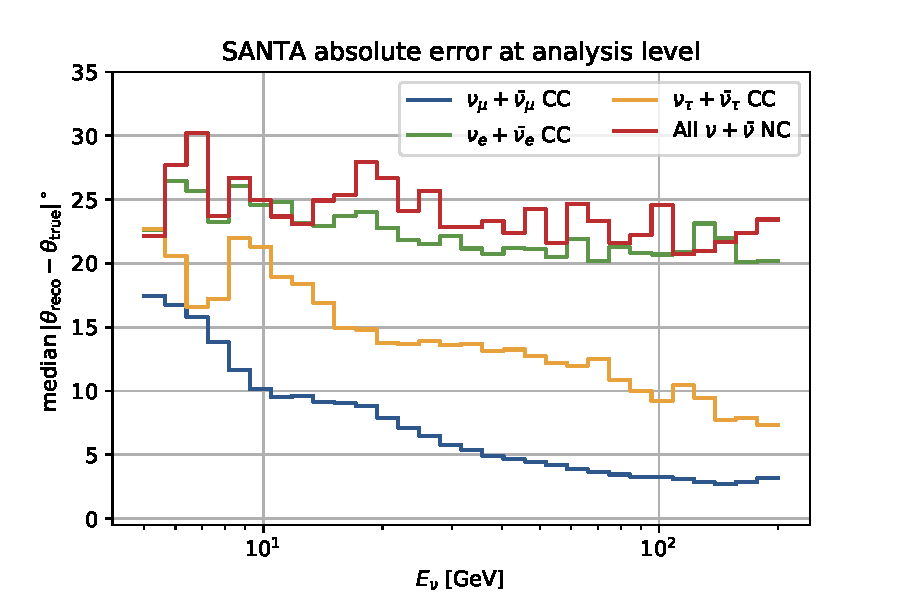
\includegraphics[width=0.8\linewidth]{figures/icecube/reconstruction/santa/santa_absolute_error_final.pdf}
    \caption{Median error on the reconstructed zenith angle at the final level of the sample selection as a function of neutrino energy.}
    \label{fig:santa-resolution}
\end{figure}

The group and phase indices of refraction depend on the wavelength, but for this reconstruction the value for a wavelength of $\lambda=400\;\mathrm{nm}$
\footnote{$400\;\mathrm{nm}$ is near the wavelength of the highest acceptance of the optical modules.\cite{icecube_detector_17}} is used, where $n_{\mathrm{gr}}=1.356$ and $n_{\mathrm{ph}}=1.319$~from~\sidecite{PRICE200197}. An example of a simulated event reconstructed with \textsc{santa} is shown in Figure~\ref{fig:santa-multi-string-example}. The solid and dashed lines show the geometric arrival time calculated according to equation~\ref{eq:t_geom-MS-track} using reconstructed and true track parameters, respectively. The circles indicate hits in DOMs, and those hits that have been removed by the hit cleaning procedure are crossed out. The median error on the zenith angle reconstructed using \textsc{SANTA} is shown in figure~\ref{fig:santa-resolution}, split by neutrino interaction type. As expected, the error is the smallest for $\nu_\mu$-CC interactions, since those produce track signatures that most closely resemble the infinite track hypothesis underlying the \textsc{SANTA} reconstruction algorithm. The worst resolution is achieved for interactions that only produce electronic or hadronic showers, since they produce cascade signatures hardly resembling the infinite track assumption. It is also apparent that the median resolution for $\nu_\tau$-CC events lies between that of $\nu_\mu$-CC events and pure cascade events. This is readily explained by the fact that 17\% of these interactions also produce a muon in their final state.

In addition to the zenith angle reconstruction, SANTA can also be used to fit a simplified cascade hypothesis to the observed hits. For this purpose, it is assumed that light is emitted uniformly in all directions originating from the interaction vertex as shown in the left panel in figure~\ref{fig:idealized_signatures}. With this assumption of perfect rotational symmetry, it is not possible to reconstruct a direction, and the cascade is fully characterized by the position of the vertex and the interaction time. The ratio of the $\chi^2$ of the infinite-track regression and the $\chi^2$ of this \emph{cascade-only} regression is used as a proxy for the neutrino flavor in this analysis. If it is smaller than one, the infinite-track hypothesis achieves a better fit to the data than the cascade-only hypothesis.

\subsubsection{Energy reconstruction}
\label{sec:leera}
The energy reconstruction runs as a separate step after the zenith angle reconstruction. In contrast to \textsc{SANTA}, the energy reconstruction fits a combined hypothesis consisting of a cascade and a finite-length track originating at the same point of the cascade. Both the cascade and the track are constrained to move only along the infinite track that has been fit in the zenith reconstruction. This means that the model fit in the energy reconstruction is fully characterized by the shift of the vertex along the infinite track, the length of the finite track (which is linearly related to the track energy), and the energy of the cascade. Given these parameters, the expected light yield for all DOMs is calculated using the so-called \emph{photonics tables}. The tables consist of B-spline coefficients that have been fit to simulated photon propagation for cascades and 3~m long tracks segments at different depths and directions inside the IceCube array to give a (time-dependent) expectation value for the photon count at arbitrary positions inside the detector. The expectation of an arbitrarily long track is calculated by chaining the 3~m segments together that fully cover the desired track length, and scaling the amplitude of the last segment by the remainder of the division of the desired length by the length of the segments. Given these expectation values as a function of event parameters, $\lambda_i(\theta)$, for every DOM, $i$, a simple Poisson ''hit vs. no-hit'' log-likelihood is calculated as
\begin{equation}
    \log(\mathcal{L}) = \sum_{i\in\mathrm{DOMs\;without\;hits}} e^{-\lambda_i(\theta)} + \sum_{i\in\mathrm{DOMs\;with\;hits}} (1 - e^{-\lambda_i(\theta)})\;.
    \label{eq:leera-llh}
\end{equation}
This likelihood is maximized under the hypothesis that the shift, track length, and cascade energy are all free parameters, and under the alternative hypothesis where the track length is fixed to zero, the latter of which corresponds to a cascade-only hypothesis. The difference between these two log-likelihoods provides a measure of the degree to which the combined track and cascade hypothesis fits the observed data better than a track-only hypothesis. It is one of the inputs that is used in a BDT to calculate an overall score of how track-like an observed event signature is. The median relative error in the reconstructed total energy (that is, the sum of the track energy and the cascade energy) is shown in Figure~\ref{fig:leera-resolution}. As with the zenith angle reconstruction, the relative error is smallest for \numucc-events. This is expected, since these events fit the hypothesis of an initial cascade combined with a finite track the best. The second-best resolution is achieved for $\nu_{e,\mathrm{CC}}$-events, while it is poorest for $\nu_{\tau,\mathrm{CC}}$ and neutral-current events. This is explained by the fact that the expected light yield that is put in Equation~\ref{eq:leera-llh} is based on the assumption that all particles that are produced in the interaction are visible to the detector. While this assumption is a good approximation for $\nu_{e,\mathrm{CC}}$-events, it does not hold for hadronic cascades that contain some neutral components as discussed in chapter~\ref{sec:had-showers}. The true energy of the primary particles that produce hadronic cascades is therefore systematically under-estimated and has a larger uncertainty. This additional uncertainty is fundamentally irreducible, because it is not possible to distinguish the signatures of hadronic and electromagnetic showers.

\begin{figure}
    \centering
    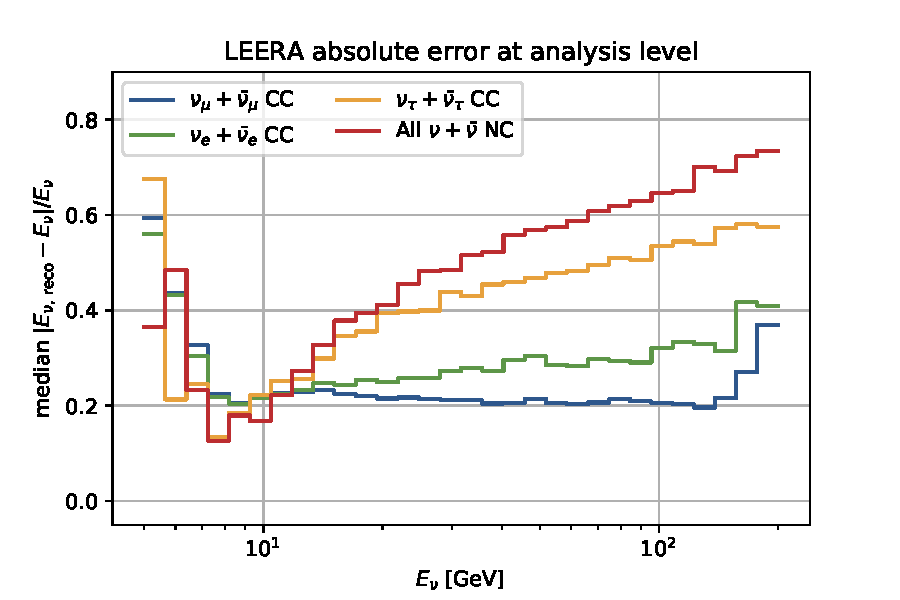
\includegraphics[width=0.8\linewidth]{figures/icecube/reconstruction/leera/leera_absolute_error_final.pdf}
    \caption{Median fractional error on the reconstructed energy at the final level of the sample selection as a function of neutrino energy.}
    \label{fig:leera-resolution}
\end{figure}

\subsection{Signature Classification}
\label{sec:pid}
In addition to the energy and zenith angle, the measurement presented in this thesis requires a score that separates track-like \numucc-events from other types of interaction. While previous analyses used only single variables such as the reconstructed track length to differentiate between tracks and cascades~\cite{deepcore_sterile_2017, Aartsen_2015,IceCube:2019dqi}, the analysis presented in this thesis uses several variables as input into a Boosted Decision-Tree (BDT) to compute a score for how track-like the observed signature is. The BDT classifier is taken from the \texttt{scikit-learn}\cite{scikit-learn} package and trained to classify between tracks and cascades using the following input variables:
\begin{itemize}
    \item SANTA $\chi^2\textrm{-ratio}$, defined as  $\frac{(\chi^{2}/\mathrm{d.o.f.})_{\mathrm{track}}}{(\chi^{2}/\mathrm{d.o.f.})_{\mathrm{cascade}}}$, i.e. the ratio of goodness-of-fit metrics from each fit hypothesis in the directional reconstruction (see section \ref{sec:santa})
    \item $\Delta$LLH from energy reconstruction, defined as LLH$_\mathrm{track}-$LLH$_\mathrm{cascade}$, i.e. the best-fit LLH value from each hypothesis (see section \ref{sec:leera})
    \item Reconstructed muon track length, $L_{\mu}$
    \item Radial distance of the reconstructed interaction vertex from string 36\footnote{String 36 is approximately at the center of the array, and near to the densest region of DeepCore (see Fig.~\ref{fig:icecube-schematic}).}, $\rho^{36}_{vertex}$
    \item Radial distance of the end-point from string 36, $\rho^{36}_{stop}$
    \item Depth of the interaction vertex, $z_{vertex}$
    \item Depth of the end point, $z_{stop}$    
\end{itemize}
\begin{figure*}
    \centering
    \ref{leera_pid_legend}

    
    \tikzsetnextfilename{santa_pid_prefit}%
\begin{tikzpicture}
    \pgfplotstableread{figures/icecube/classification/variables/SANTA_PID.csv}\table
    \begin{groupplot}[
        xmin=-0.25,xmax=5.25,
        xmode=normal,
        xmajorgrids, ymajorgrids,
        width=0.45\linewidth,
        ylabel style={at={(-0.15,0.5)}},
        group/.cd,
        group size=1 by 2,
        xticklabels at=edge bottom,
        vertical sep=10pt
        ]
    \nextgroupplot[
        height=0.35\linewidth,
        legend cell align={left},
        legend columns=4,
        legend to name=santa_pid_legend,
        ymode=log,
        ymin=5.937489735229232e-11, ymax=0.05052335190265824,
        ylabel=rate (Hz),
        % add magic filter to correctly handle empty bins in logarithmic y-axes:
        % If a bin-count is too low or zero, it would cause the line to be
        % interrupted, which creates artefacts and ugliness. Instead, we replace
        % these bin-counts with values that are just below the axis limit.
        % Because of the way pgfplots works, the input is the raw number but the
        % output has to be the log. Weird, I know.
        y filter/.expression={y < 5.937489735229232e-11 ? ln(5.937489735229232e-12) : ln(y)}
    ]

    % \ploterrorband[muon_color]{muon}{1}
    % \addlegendentry{atm. muons}

    % \ploterrorband[nue_color]{nuenuebar}{1}
    % \addlegendentry{$\nu_e + \bar{\nu}_e$}

    % \ploterrorband[numu_color]{numunumubar}{1}
    % \addlegendentry{$\nu_\mu + \bar{\nu}_\mu$}

    % \ploterrorband[nutau_color]{nutaunutaubar}{1}
    % \addlegendentry{$\nu_\tau + \bar{\nu}_\tau$}


    % alternative event breakdown by interaction
    \ploterrorband[nue_color]{nue_ccnuebar_cc}{1}
    \addlegendentry{$\nu_e + \bar{\nu}_e$, CC}
    
    \ploterrorband[numu_color]{numu_ccnumubar_cc}{1}
    \addlegendentry{$\nu_\mu + \bar{\nu}_\mu$, CC}
    
    \ploterrorband[nutau_color]{nutau_ccnutaubar_cc}{1}
    \addlegendentry{$\nu_\tau + \bar{\nu}_\tau$, CC}
    
    \ploterrorband[nc_color]{nuall_ncnuallbar_nc}{1}
    \addlegendentry{all $\nu$, NC}

    \ploterrorband{total_mc}{1}
    \addlegendentry{total MC}

    \addplot[
        mark=*,
        mark options={scale=0.5, fill=black},
        black,
        only marks,
        error bars/.cd,
        x dir=none,
        y dir=both,
        y explicit
    ] table [x=bin_midpoints, y=data, y error=data__err]  from \table;
    \addlegendentry{data}


    \nextgroupplot[
        height=0.2\linewidth,
        ymin=0.5, ymax=1.5,
        ylabel=data/MC ratio,
        xlabel=SANTA $\chi^2\textrm{-ratio}$
    ]

    \ploterrorband{data_mc_ratio}{1}
    % \ploterrorband[numu_color]{numu_ccnumubar_cc_frac}{1}
    \end{groupplot}
\end{tikzpicture}

    \tikzsetnextfilename{leera_pid_prefit}%
\begin{tikzpicture}
    \pgfplotstableread{figures/icecube/classification/variables/LEERA_PID.csv}\table
    \begin{groupplot}[
        xmin=-22.0,xmax=22.0,
        xmode=normal,
        xmajorgrids, ymajorgrids,
        width=0.45\linewidth,
        ylabel style={at={(-0.15,0.5)}},
        group/.cd,
        group size=1 by 2,
        xticklabels at=edge bottom,
        vertical sep=10pt
        ]
    \nextgroupplot[
        height=0.35\linewidth,
        legend cell align={left},
        legend columns=4,
        legend to name=leera_pid_legend,
        ymode=log,
        ymin=4.429678646618006e-09, ymax=5e-3,
        ylabel=rate (Hz),
        % add magic filter to correctly handle empty bins in logarithmic y-axes:
        % If a bin-count is too low or zero, it would cause the line to be
        % interrupted, which creates artefacts and ugliness. Instead, we replace
        % these bin-counts with values that are just below the axis limit.
        % Because of the way pgfplots works, the input is the raw number but the
        % output has to be the log. Weird, I know.
        y filter/.expression={y < 4.429678646618006e-09 ? ln(4.429678646618006e-10) : ln(y)}
    ]

    % \ploterrorband[muon_color]{muon}{1}
    % \addlegendentry{atm. muons}

    % \ploterrorband[nue_color]{nuenuebar}{1}
    % \addlegendentry{$\nu_e + \bar{\nu}_e$}

    % \ploterrorband[numu_color]{numunumubar}{1}
    % \addlegendentry{$\nu_\mu + \bar{\nu}_\mu$}

    % \ploterrorband[nutau_color]{nutaunutaubar}{1}
    % \addlegendentry{$\nu_\tau + \bar{\nu}_\tau$}


    % alternative event breakdown by interaction
    \ploterrorband[nue_color]{nue_ccnuebar_cc}{1}
    \addlegendentry{$\nu_e + \bar{\nu}_e$, CC}
    
    \ploterrorband[numu_color]{numu_ccnumubar_cc}{1}
    \addlegendentry{$\nu_\mu + \bar{\nu}_\mu$, CC}
    
    \ploterrorband[nutau_color]{nutau_ccnutaubar_cc}{1}
    \addlegendentry{$\nu_\tau + \bar{\nu}_\tau$, CC}
    
    \ploterrorband[nc_color]{nuall_ncnuallbar_nc}{1}
    \addlegendentry{all $\nu$, NC}

    \ploterrorband{total_mc}{1}
    \addlegendentry{total MC}

    \addplot[
        mark=*,
        mark options={scale=0.5, fill=black},
        black,
        only marks,
        error bars/.cd,
        x dir=none,
        y dir=both,
        y explicit
    ] table [x=bin_midpoints, y=data, y error=data__err]  from \table;
    \addlegendentry{data}


    \nextgroupplot[
        height=0.2\linewidth,
        ymin=0.5, ymax=1.5,
        ylabel=data/MC ratio,
        xlabel=LLH$_\mathrm{track}-$LLH$_\mathrm{cascade}$
    ]

    \ploterrorband{data_mc_ratio}{1}
    % \ploterrorband[numu_color]{numu_ccnumubar_cc_frac}{1}
    \end{groupplot}
\end{tikzpicture}

    \caption{Distribution and data/MC comparison for the two most important input variables into the classification BDT.}
    \label{fig:bdt-input-vars}
\end{figure*}
Of these variables, the SANTA $\chi^2\textrm{-ratio}$ and $\Delta$LLH contribute the most to the final score. Their distributions and comparison between data and simulation can be seen in figure\ref{fig:bdt-input-vars} at the L5 selection level, where neutrinos are weighted with \textsc{NuFit}~4.0\cite{nufit40} global fit parameters.
The training data consists of simulated $\nu_e$-CC interactions and neutral-current interactions representing cascades, and $\nu_\mu$-CC interactions representing tracks. Tau neutrino interactions are not included in the training data in order to avoid confusion due to the 17\% of $\nu_\tau$-CC interactions that produce track-like signatures. The training samples are weighted to approximate the neutrino flux expected from the HKKM model~\sidecite{Honda:2015fha} \emph{without} oscillations. The distributions for these variables for tracks and cascades as they were used in training can be found in the Appendix~\ref{sec:apx-pidvars}. To guard against over-training of the classifier, only half of the available simulation is used for training, while the other half is held out for validation. The output score of the classifier is referred to as \emph{particle-ID} (PID) and ranges from zero (very cascade-like) to one (very track-like). The distribution of the PID score for simulated neutrino interactions is shown in figure~\ref{fig:pid-score}, broken down by flavor and interaction type. The distributions are individually normalized to help visualize the shape differences between the different neutrino interactions. The distributions for all interaction types show a large peak around a probability score of 0.5, suggesting that the event signature cannot be clearly classified for the majority of events. A second peak exists only in the distribution of $\nu_\mu$-CC events close to a score of one, meaning that there exists a population of these events that can be very clearly classified as being track-like. There also exists some excess of high PID values in the distribution of $\nu_\tau$-CC events corresponding to those events where the decay of the tauon produces a muon. Notably, there is no population of events that can be cleanly classified as a cascade event, i.e., there are no PID scores close to zero. The reason for this is that the two classes are nested hypotheses, one containing only a cascade and the other containing a combination of a cascade and a track, and it is never possible to prove that a cascade-like signature does not contain at least a short track segment.
\begin{figure}
    \centering
    %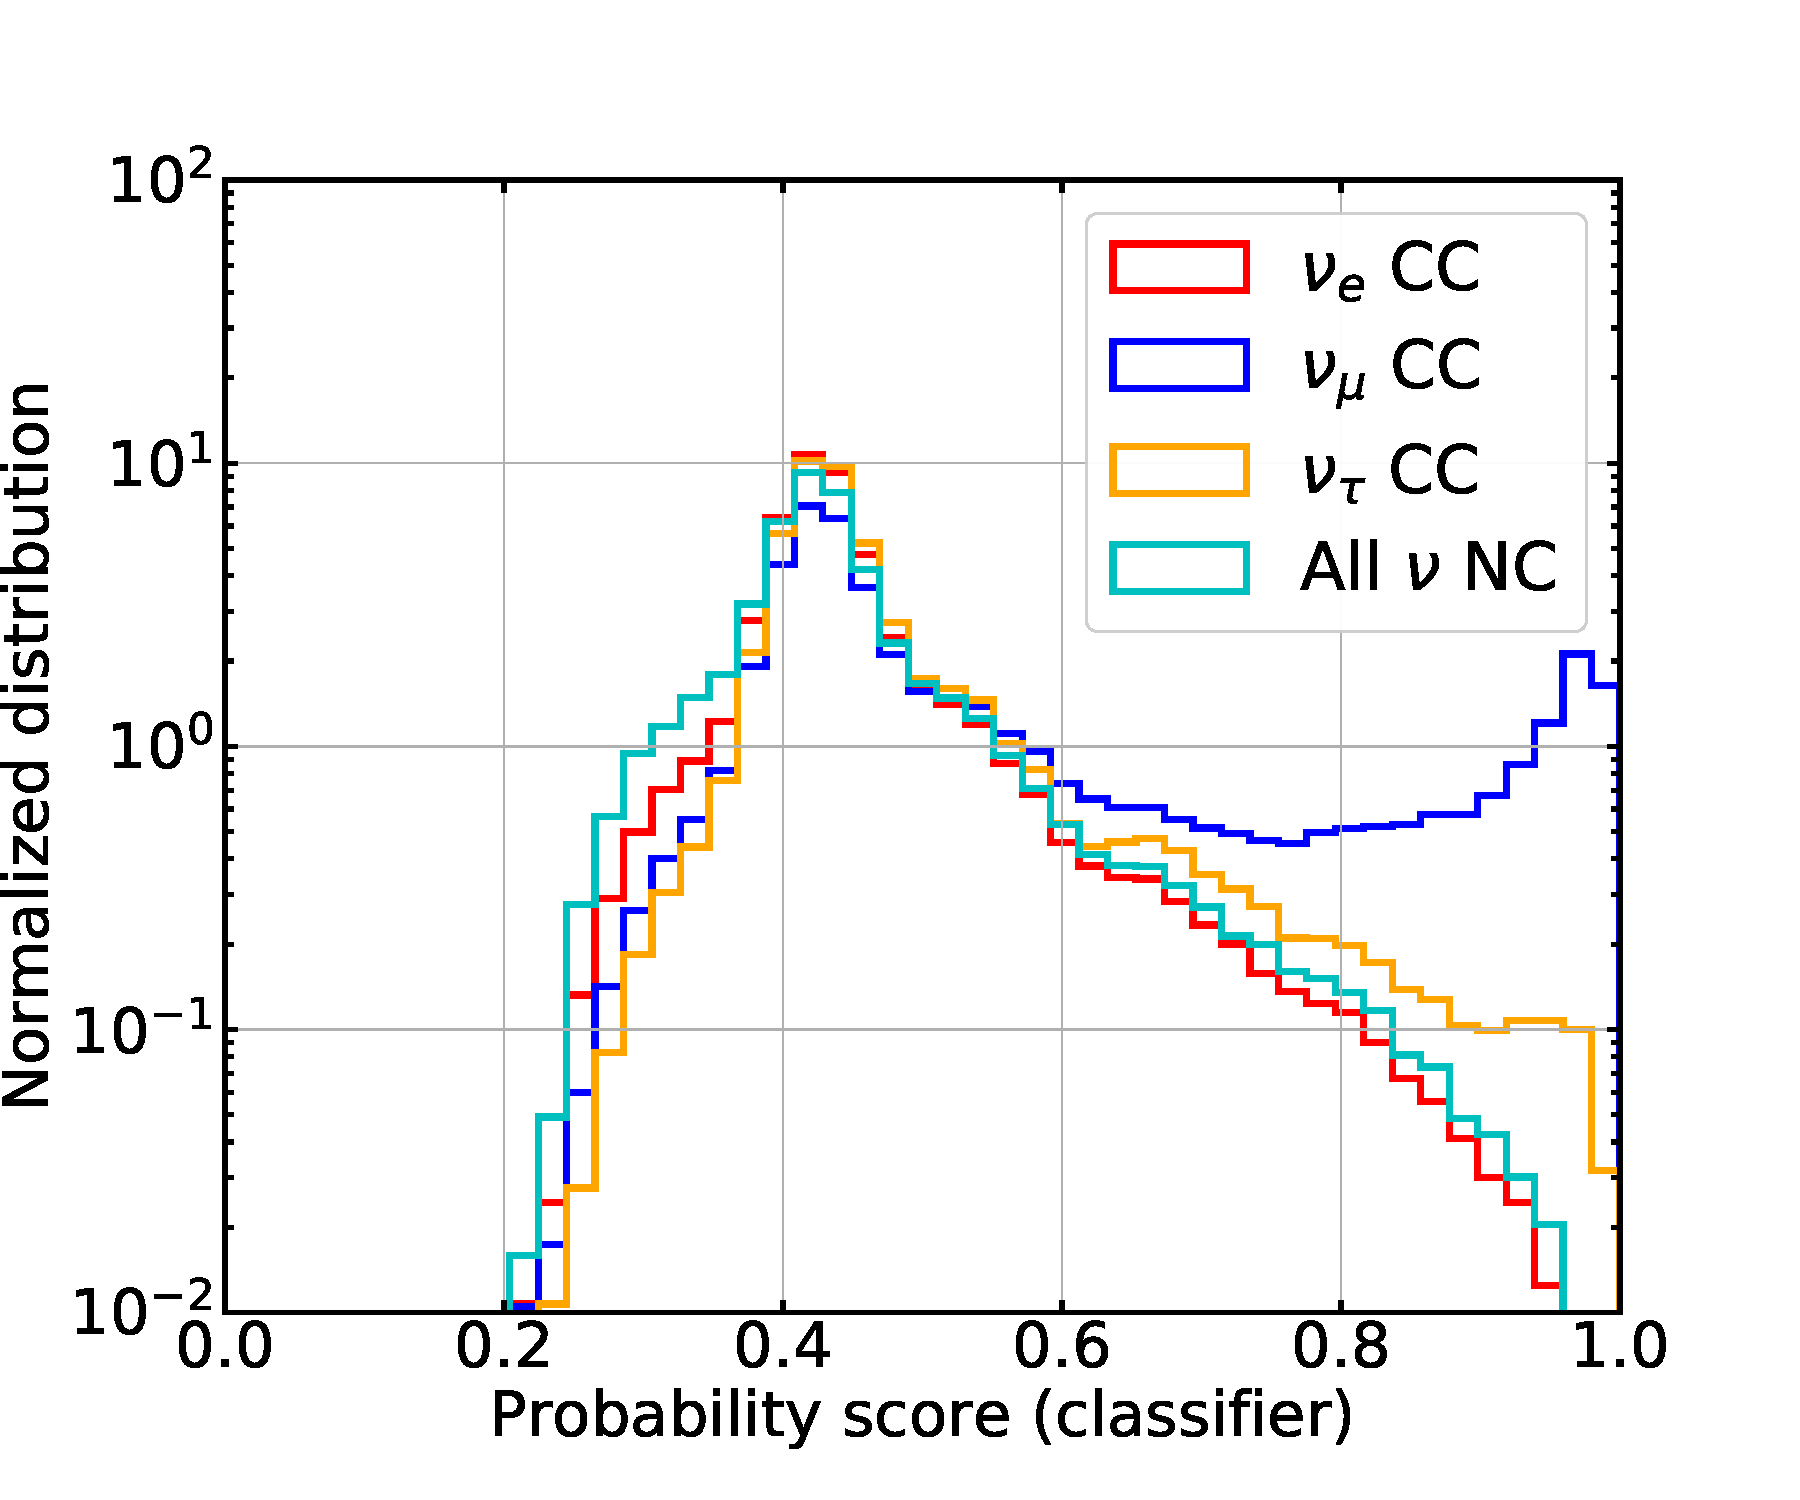
\includegraphics[width=0.8\linewidth]{figures/icecube/classification/bdt_score_normalized.pdf}
    \tikzsetnextfilename{bdt_score_normalized}%
\begin{tikzpicture}

    \pgfplotstableread{figures/icecube/classification/gbm_normalized_nu_hists_nufit22.csv}\table
    \begin{axis}[
        xmin=0,xmax=1.0,
        xmajorgrids, ymajorgrids,
        width=0.7\linewidth,
        height=0.6\linewidth,
        ymode=log,
        ymin=1e-02, ymax=100,
        ylabel=distribution density,
        xlabel=BDT score,
        legend cell align={left},
        legend columns=2,
    ]

    \addplot[const plot, nue_color, thick] table [x=bin_edges, y=nue_cc] from \table;
    \addlegendentry{$\nu_e + \bar{\nu}_e$, CC}
    \addplot[const plot, numu_color, thick] table [x=bin_edges, y=numu_cc] from \table;
    \addlegendentry{$\nu_\mu + \bar{\nu}_\mu$, CC}
    \addplot[const plot, nutau_color, thick] table [x=bin_edges, y=nutau_cc] from \table;
    \addlegendentry{$\nu_\tau + \bar{\nu}_\tau$, CC}
    \addplot[const plot, nc_color, thick] table [x=bin_edges, y=nu_nc] from \table;
    \addlegendentry{all $\nu$, NC}
    
    \end{axis}
\end{tikzpicture}

    \caption{PID score distribution for simulated neutrino events at the final level of the event selection, weighted according to the HKKM flux model~\cite{Honda:2015fha} and neutrino oscillations with \textsc{NuFit}~4.0\cite{nufit40} global fit parameters, normalized to unity.}
    \label{fig:pid-score}
\end{figure}

\subsection{Final Sample Selection}

After the reconstruction and classification step, several final cut variables are applied to reduce the background of atmospheric muons to only a few percent, and to remove a small number of events from data containing coincident muons. These cuts are:
\begin{itemize}
    \item The reconstruction of energy and zenith angle has to be successful. This requires, in particular, that at least five hits remain after the hit cleaning procedure described in Section~\ref{sec:santa}.
    \item The reconstructed energy should be in the range $6;\mathrm{GeV} < E_{\mathrm{reco}} < 156\;\mathrm{GeV}$.
    \item Require a minimum PID score (see section~\ref{sec:pid}) of 0.55 to only include at least somewhat track-like events.
    \item Reconstructed $\cos(\theta_z) < 0.1$ to remove events that enter the detector from above the horizon.
    \item Require a minimum goodness-of-fit of the zenith reconstruction with $\chi^2_{\mathrm{mod}}/\mathrm{d.o.f.} < 50$.
    \item A tighter cut on the L4 muon BDT score (see section~\ref{sec:level4-selection}) of $P_\nu > 0.97$.
    \item Fewer than eight hits in the outermost strings of the IceCube array, and a positive "z-travel" value for hits in the uppermost 15 layers of DOMs in the (non-DeepCore) IceCube array. The "z-travel" value for a given sequence of hits is calculated by subtracting the mean value of the z-coordinate of the first quartile of hits from the mean z-coordinate of all hits. 
\end{itemize}

\begin{figure}
    \centering
    \tikzsetnextfilename{z_travel_top15}%
\begin{tikzpicture}
    \pgfplotstableread{figures/icecube/selection/Level7/z_travel_top15.csv}\table

    \begin{axis}[
    	xmin=-150,xmax=150,
        xmode=normal,
        xmajorgrids, ymajorgrids,
        width=0.45\linewidth,
        % ylabel style={at={(-0.15,0.5)}},
        height=0.55\linewidth,
        legend cell align={left},
        legend columns=3,
        ymode=log,
        ymin=2e-9, ymax=5e-6,
        y filter/.expression={y < 1e-10 ? ln(1e-11) : ln(y)},
        ylabel=rate (Hz),
        xlabel=z-travel in upper 15 IceCube DOMs
    ]
	
    \ploterrorband[muon_color]{muon}{1}
    \addlegendentry{atm. muons}

    \ploterrorband[nue_color]{nuenuebar}{1}
    \addlegendentry{$\nu_e + \bar{\nu}_e$}
    
    \ploterrorband[numu_color]{numunumubar}{1}
    \addlegendentry{$\nu_\mu + \bar{\nu}_\mu$}
    
    \ploterrorband[nutau_color]{nutaunutaubar}{1}
    \addlegendentry{$\nu_\tau + \bar{\nu}_\tau$}
   
    
    \ploterrorband{total_mc}{1}
    \addlegendentry{total MC}
	
	
	% draw cut
    % use "axis cs" to give coordinates in the data coordinate system!
    \draw[thick,dashed] (axis cs:0,1e-9) -- (axis cs:0,5e-5);
    \draw[-stealth, very thick] (axis cs:0,3e-7)  -- node[anchor=south]{\footnotesize\sffamily signal} (axis cs:50,3e-7);
    
    \addplot[
        mark=*,
        mark options={scale=0.5, fill=black},
        black,
        only marks,
        error bars/.cd,
        x dir=none,
        y dir=both,
        y explicit
    ] table [x=bin_midpoints, y=data, y error=data__err]  from \table;
    \addlegendentry{data}
	
	\end{axis}
\end{tikzpicture}

    \caption{Distribution of the "z-travel" variable calculated for the uppermost 15 layers of IceCube DOMs. Only events with at least 4 hits in the uppermost 15 layers of DOMs are included in the histogram.}
    \label{fig:z_travel_distribution}
\end{figure}

% \begin{figure}
%     \centering
%     \tikzsetnextfilename{santa_chi2dof}%
\begin{tikzpicture}
    \pgfplotstableread{figures/icecube/selection/Level7/santa_chi2dof.csv}\table
    \begin{groupplot}[
        xmin=3,xmax=300,
        xmode=log,
        xmajorgrids, ymajorgrids,
        width=0.45\linewidth,
        ylabel style={at={(-0.15,0.5)}},
        group/.cd,
        group size=1 by 2,
        xticklabels at=edge bottom,
        vertical sep=10pt
        ]
    \nextgroupplot[
        height=0.3\linewidth,
        legend cell align={left},
        legend columns=3,
        legend to name=santa_chi2dof_legend,
        ymode=log,
        ymin=2e-8, ymax=5e-3,
        ylabel=rate (Hz),
    ]

    \ploterrorband[muon_color]{muon}{1}
    \addlegendentry{atm. muons}

    \ploterrorband[nue_color]{nuenuebar}{1}
    \addlegendentry{$\nu_e + \bar{\nu}_e$}
    
    \ploterrorband[numu_color]{numunumubar}{1}
    \addlegendentry{$\nu_\mu + \bar{\nu}_\mu$}
    
    \ploterrorband[nutau_color]{nutaunutaubar}{1}
    \addlegendentry{$\nu_\tau + \bar{\nu}_\tau$}
    
    % alternative  event breakdown by interaction
    
    % \ploterrorband[nue_color]{nue_ccnuebar_cc}{1}
    % \addlegendentry{$\nu_e + \bar{\nu}_e$, CC}
    
    % \ploterrorband[numu_color]{numu_ccnumubar_cc}{1}
    % \addlegendentry{$\nu_\mu + \bar{\nu}_\mu$, CC}
    
    % \ploterrorband[nutau_color]{nutau_ccnutaubar_cc}{1}
    % \addlegendentry{$\nu_\tau + \bar{\nu}_\tau$, CC}
    
    % \ploterrorband[nc_color]{nuall_ncnuallbar_nc}{1}
    % \addlegendentry{all $\nu$, NC}
    
    \ploterrorband{total_mc}{1}
    \addlegendentry{total MC}

    % draw cut
    % use "axis cs" to give coordinates in the data coordinate system!
    \draw[thick,dashed] (axis cs:50,1e-8) -- (axis cs:50,5e-4);
    \draw[-stealth, very thick] (axis cs:50,1e-7)  -- node[anchor=south]{\footnotesize\sffamily signal} (axis cs:20,1e-7);
    
    \addplot[
        mark=*,
        mark options={scale=0.5, fill=black},
        black,
        only marks,
        error bars/.cd,
        x dir=none,
        y dir=both,
        y explicit
    ] table [x=bin_midpoints, y=data, y error=data__err]  from \table;
    \addlegendentry{data}


    \nextgroupplot[
        height=0.2\linewidth,
        ymin=0.8, ymax=1.2,
        ylabel=data/MC ratio,
        xlabel=SANTA $\chi^2 / \mathrm{d.o.f.}$\strut
    ]
    
    \ploterrorband{data_mc_ratio}{1}
    %\plotratioerrorband[muon_color]{muon}{total_mc}
    \end{groupplot}
\end{tikzpicture}

%     \caption{Distribution of the SANTA goodness-of-fit variable.}
%     \label{fig:santa_chi2dof_distribution}
% \end{figure}


\begin{figure*}
    \centering
    \ref{reco_coszen_legend}\par
    \tikzsetnextfilename{santa_chi2dof}%
\begin{tikzpicture}
    \pgfplotstableread{figures/icecube/selection/Level7/santa_chi2dof.csv}\table
    \begin{groupplot}[
        xmin=3,xmax=300,
        xmode=log,
        xmajorgrids, ymajorgrids,
        width=0.45\linewidth,
        ylabel style={at={(-0.15,0.5)}},
        group/.cd,
        group size=1 by 2,
        xticklabels at=edge bottom,
        vertical sep=10pt
        ]
    \nextgroupplot[
        height=0.3\linewidth,
        legend cell align={left},
        legend columns=3,
        legend to name=santa_chi2dof_legend,
        ymode=log,
        ymin=2e-8, ymax=5e-3,
        ylabel=rate (Hz),
    ]

    \ploterrorband[muon_color]{muon}{1}
    \addlegendentry{atm. muons}

    \ploterrorband[nue_color]{nuenuebar}{1}
    \addlegendentry{$\nu_e + \bar{\nu}_e$}
    
    \ploterrorband[numu_color]{numunumubar}{1}
    \addlegendentry{$\nu_\mu + \bar{\nu}_\mu$}
    
    \ploterrorband[nutau_color]{nutaunutaubar}{1}
    \addlegendentry{$\nu_\tau + \bar{\nu}_\tau$}
    
    % alternative  event breakdown by interaction
    
    % \ploterrorband[nue_color]{nue_ccnuebar_cc}{1}
    % \addlegendentry{$\nu_e + \bar{\nu}_e$, CC}
    
    % \ploterrorband[numu_color]{numu_ccnumubar_cc}{1}
    % \addlegendentry{$\nu_\mu + \bar{\nu}_\mu$, CC}
    
    % \ploterrorband[nutau_color]{nutau_ccnutaubar_cc}{1}
    % \addlegendentry{$\nu_\tau + \bar{\nu}_\tau$, CC}
    
    % \ploterrorband[nc_color]{nuall_ncnuallbar_nc}{1}
    % \addlegendentry{all $\nu$, NC}
    
    \ploterrorband{total_mc}{1}
    \addlegendentry{total MC}

    % draw cut
    % use "axis cs" to give coordinates in the data coordinate system!
    \draw[thick,dashed] (axis cs:50,1e-8) -- (axis cs:50,5e-4);
    \draw[-stealth, very thick] (axis cs:50,1e-7)  -- node[anchor=south]{\footnotesize\sffamily signal} (axis cs:20,1e-7);
    
    \addplot[
        mark=*,
        mark options={scale=0.5, fill=black},
        black,
        only marks,
        error bars/.cd,
        x dir=none,
        y dir=both,
        y explicit
    ] table [x=bin_midpoints, y=data, y error=data__err]  from \table;
    \addlegendentry{data}


    \nextgroupplot[
        height=0.2\linewidth,
        ymin=0.8, ymax=1.2,
        ylabel=data/MC ratio,
        xlabel=SANTA $\chi^2 / \mathrm{d.o.f.}$\strut
    ]
    
    \ploterrorband{data_mc_ratio}{1}
    %\plotratioerrorband[muon_color]{muon}{total_mc}
    \end{groupplot}
\end{tikzpicture}

    \tikzsetnextfilename{reco_coszen_l5}%
\begin{tikzpicture}
    \pgfplotstableread{figures/icecube/selection/Level7/reco_coszen.csv}\table
    \begin{groupplot}[
        xmin=-1.1,xmax=1.1,
        xmode=normal,
        xmajorgrids, ymajorgrids,
        width=0.45\linewidth,
        ylabel style={at={(-0.15,0.5)}},
        group/.cd,
        group size=1 by 2,
        xticklabels at=edge bottom,
        vertical sep=10pt
        ]
    \nextgroupplot[
        height=0.3\linewidth,
        legend cell align={left},
        legend columns=-1,
        legend to name=reco_coszen_legend,
        ymode=log,
        ymin=2e-7, ymax=5e-4,
        ylabel=rate (Hz),
        % add magic filter to correctly handle empty bins in logarithmic y-axes:
        % If a bin-count is too low or zero, it would cause the line to be
        % interrupted, which creates artefacts and ugliness. Instead, we replace
        % these bin-counts with values that are just below the axis limit.
        % Because of the way pgfplots works, the input is the raw number but the
        % output has to be the log. Weird, I know.
        y filter/.expression={y < 8.7587858920556e-09 ? ln(8.758785892055601e-10) : ln(y)}
    ]

    \ploterrorband[muon_color]{muon}{1}
    \addlegendentry{atm. muons}

    \ploterrorband[nue_color]{nuenuebar}{1}
    \addlegendentry{$\nu_e + \bar{\nu}_e$}

    \ploterrorband[numu_color]{numunumubar}{1}
    \addlegendentry{$\nu_\mu + \bar{\nu}_\mu$}

    \ploterrorband[nutau_color]{nutaunutaubar}{1}
    \addlegendentry{$\nu_\tau + \bar{\nu}_\tau$}


    % alternative event breakdown by interaction
    % \ploterrorband[nue_color]{nue_ccnuebar_cc}{1}
    % \addlegendentry{$\nu_e + \bar{\nu}_e$, CC}
    %
    % \ploterrorband[numu_color]{numu_ccnumubar_cc}{1}
    % \addlegendentry{$\nu_\mu + \bar{\nu}_\mu$, CC}
    %
    % \ploterrorband[nutau_color]{nutau_ccnutaubar_cc}{1}
    % \addlegendentry{$\nu_\tau + \bar{\nu}_\tau$, CC}
    %
    % \ploterrorband[nc_color]{nuall_ncnuallbar_nc}{1}
    % \addlegendentry{all $\nu$, NC}

    \ploterrorband{total_mc}{1}
    \addlegendentry{total MC}

    \ploterrorbar{data}
    \addlegendentry{data}


    % draw cut
    % use "axis cs" to give coordinates in the data coordinate system!
    \draw[thick,dashed] (axis cs:0.1,1e-9) -- (axis cs:0.1,5e-4);
    \draw[-stealth, very thick] (axis cs:0.1,1e-4)  -- node[anchor=south]{\footnotesize\sffamily signal} (axis cs:-0.4,1e-4);
    
    \nextgroupplot[
        height=0.2\linewidth,
        ymin=0.5, ymax=1.5,
        ylabel=data/MC ratio,
        xlabel=reconstructed $\cos(\theta_{\mathrm{zenith}})$\strut
    ]

    \ploterrorband{data_mc_ratio}{1}
    \end{groupplot}
\end{tikzpicture}

    \caption{Distribution of the SANTA goodness-of-fit variable and the reconstructed zenith angle at L5 of the event selection process.}
    \label{fig:final_cut_vars_l5}
\end{figure*}

The cuts on energy, zenith angle, and PID define the range of the binning that will be used in the analysis. The cut on the zenith angle in particular is applied not only to reduce the background of atmospheric muons, but also to remove the phase space of neutrino events where muons that are produced in the same air shower that also produced the neutrino cause it to be vetoed by the muon filter cuts. This effect is referred to as the "self-veto" effect and would lead to a disagreement between data and simulation since coincident muons are never simulated. The distribution of the cosine of the reconstructed zenith angle is shown in the right panel of figure~\ref{fig:final_cut_vars_l5}, and it is apparent from the distributions that atmospheric muons dominate in the region of down-going events.

The requirement on the SANTA goodness-of-fit not only ensures that the included events are well-reconstructed, but also reduces the fraction of muons in the sample, as can be seen from the distributions shown in the left panel of figure~\ref{fig:final_cut_vars_l5}. The number of hits on the outermost strings and the "z-travel" variable calculated for hits in the uppermost 15 layers of IceCube DOMs are indicators of muons that hit the detector within the trigger window of a neutrino event. Such coincidences are entirely absent in simulation, which becomes especially apparent in the distribution of the "z-travel" variable shown in figure~\ref{fig:z_travel_distribution}, where a negative value indicates a down-going signal. After the application of all these cuts, the data sample consists of well-reconstructed, track-like events with an expected background from atmospheric muons of only $\sim 2\%$ as shown in table~\ref{tab:muon-rejection-cut-rates}.

\begin{table}
\caption{Successively applied cuts on the data sample. The bottom row corresponds to the final rates in the sample after all cuts have been applied. The total rate of the data and simulation does not match, which is expected since there is a large amount of uncertainty in the total normalization. Muon contamination is the muon rate divided by the total event rate. Numbers calculated at the NuFit 4.0 global best-fit point.}
\centering
\begin{tabular}{@{}lrrrr@{}}\toprule
& \multicolumn{3}{c}{rate ($\mu$Hz)} & \\ \cmidrule{2-4}
cut                                 & $\nu$ (sim) & $\mu$ (sim) & data & $\mu$ fraction \\ \midrule
event has SANTA reco                   & 957  & 314  & 1183 & 24.7\%  \\
event within energy range              & 862  & 311  & 1095 & 26.5\%  \\
BDT score $>0.55$                      & 232  & 117  &  336 & 33.5\%  \\
$\cos(\theta_{\mathrm{reco}}) < 0.1$   & 175  &  17  &  177 & 8.8\%   \\
SANTA $\chi^2/\mathrm{d.o.f.} < 50$    & 164  &  12  &  161 & 6.6\%   \\
L4 muon $\nu$ prob $> 0.97$            & 101  &   2  &   93 & 2.1\% \\
\midrule\addlinespace
coinc. $\mu$ cuts (final rate) & \textbf{101} & \textbf{2} & \textbf{93} & \textbf{2.1\%
} \\ \bottomrule
\end{tabular}
\label{tab:muon-rejection-cut-rates}
\end{table}

\begin{figure*}
    \centering
    \ref{reco_coszen_prefit_legend}\par
    \begin{tikzpicture}
    \pgfplotstableread{figures/icecube/selection/final_sample_prefit/reco_coszen.csv}\table
    \begin{groupplot}[
        xmin=-1.055,xmax=0.15500000000000003,
        xmode=normal,
        xmajorgrids, ymajorgrids,
        width=0.45\linewidth,
        ylabel style={at={(-0.15,0.5)}},
        group/.cd,
        group size=1 by 2,
        xticklabels at=edge bottom,
        vertical sep=10pt
        ]
    \nextgroupplot[
        height=0.3\linewidth,
        legend cell align={left},
        legend columns=-1,
        legend to name=reco_coszen_prefit_legend,
        ymode=log,
        ymin=2.670138976548827e-09, ymax=3e-5,
        ylabel=rate (Hz),
        ytick distance=1e1,
        % add magic filter to correctly handle empty bins in logarithmic y-axes:
        % If a bin-count is too low or zero, it would cause the line to be
        % interrupted, which creates artefacts and ugliness. Instead, we replace
        % these bin-counts with values that are just below the axis limit.
        % Because of the way pgfplots works, the input is the raw number but the
        % output has to be the log. Weird, I know.
        y filter/.expression={y < 2.670138976548827e-09 ? ln(2.6701389765488273e-10) : ln(y)}
    ]

    \ploterrorband[muon_color]{muon}{1}
    \addlegendentry{atm. muons}

    \ploterrorband[nue_color]{nuenuebar}{1}
    \addlegendentry{$\nu_e + \bar{\nu}_e$}

    \ploterrorband[numu_color]{numunumubar}{1}
    \addlegendentry{$\nu_\mu + \bar{\nu}_\mu$}

    \ploterrorband[nutau_color]{nutaunutaubar}{1}
    \addlegendentry{$\nu_\tau + \bar{\nu}_\tau$}


    % alternative event breakdown by interaction
    % \ploterrorband[nue_color]{nue_ccnuebar_cc}{1}
    % \addlegendentry{$\nu_e + \bar{\nu}_e$, CC}
    %
    % \ploterrorband[numu_color]{numu_ccnumubar_cc}{1}
    % \addlegendentry{$\nu_\mu + \bar{\nu}_\mu$, CC}
    %
    % \ploterrorband[nutau_color]{nutau_ccnutaubar_cc}{1}
    % \addlegendentry{$\nu_\tau + \bar{\nu}_\tau$, CC}
    %
    % \ploterrorband[nc_color]{nuall_ncnuallbar_nc}{1}
    % \addlegendentry{all $\nu$, NC}

    \ploterrorband{total_mc}{1}
    \addlegendentry{total MC}

    \ploterrorbar{data}
    \addlegendentry{data}

    \nextgroupplot[
        height=0.2\linewidth,
        ymin=-0.1, ymax=1.8,
        ylabel=rate/total MC,
        xlabel=reconstructed $\cos(\theta_{\mathrm{zenith}})$
    ]
   
    \ploterrorbar{data_mc_ratio}
    \plotratioerrorband[muon_color]{muon}{total_mc}
    \plotratioerrorband[nue_color]{nuenuebar}{total_mc}
    \plotratioerrorband[numu_color]{numunumubar}{total_mc}
    \plotratioerrorband[nutau_color]{nutaunutaubar}{total_mc}
    
    \end{groupplot}
\end{tikzpicture}

    \tikzsetnextfilename{final_level_prefit_reco_energy}%
\begin{tikzpicture}
    \pgfplotstableread{figures/icecube/selection/final_sample_prefit/reco_energy.csv}\table
    \begin{groupplot}[
        xmin=5.362591587787688,xmax=185.61920737481475,
        xmode=log,
        xmajorgrids, ymajorgrids,
        width=0.45\linewidth,
        ylabel style={at={(-0.15,0.5)}},
        group/.cd,
        group size=1 by 2,
        xticklabels at=edge bottom,
        vertical sep=10pt
        ]
    \nextgroupplot[
        height=0.3\linewidth,
        legend cell align={left},
        legend columns=-1,
        legend to name=prefit_reco_energy_legend,
        ymode=log,
        ymin=2.670138976548827e-09, ymax=3e-5,
        ylabel=rate (Hz),
        ytick distance=1e1,
        % add magic filter to correctly handle empty bins in logarithmic y-axes:
        % If a bin-count is too low or zero, it would cause the line to be
        % interrupted, which creates artefacts and ugliness. Instead, we replace
        % these bin-counts with values that are just below the axis limit.
        % Because of the way pgfplots works, the input is the raw number but the
        % output has to be the log. Weird, I know.
        y filter/.expression={y < 9.437724466286084e-10 ? ln(9.437724466286085e-11) : ln(y)}
    ]

    \ploterrorband[muon_color]{muon}{1}
    \addlegendentry{atm. muons}

    \ploterrorband[nue_color]{nuenuebar}{1}
    \addlegendentry{$\nu_e + \bar{\nu}_e$}

    \ploterrorband[numu_color]{numunumubar}{1}
    \addlegendentry{$\nu_\mu + \bar{\nu}_\mu$}

    \ploterrorband[nutau_color]{nutaunutaubar}{1}
    \addlegendentry{$\nu_\tau + \bar{\nu}_\tau$}


    % alternative event breakdown by interaction
    % \ploterrorband[nue_color]{nue_ccnuebar_cc}{1}
    % \addlegendentry{$\nu_e + \bar{\nu}_e$, CC}
    %
    % \ploterrorband[numu_color]{numu_ccnumubar_cc}{1}
    % \addlegendentry{$\nu_\mu + \bar{\nu}_\mu$, CC}
    %
    % \ploterrorband[nutau_color]{nutau_ccnutaubar_cc}{1}
    % \addlegendentry{$\nu_\tau + \bar{\nu}_\tau$, CC}
    %
    % \ploterrorband[nc_color]{nuall_ncnuallbar_nc}{1}
    % \addlegendentry{all $\nu$, NC}

    \ploterrorband{total_mc}{1}
    \addlegendentry{total MC}

    \ploterrorbar{data}
    \addlegendentry{data}

    \nextgroupplot[
        height=0.2\linewidth,
        ymin=-0.1, ymax=1.8,
        ylabel=rate/total MC,
        xlabel=reconstructed energy (GeV)
    ]

    \ploterrorbar{data_mc_ratio}
    \plotratioerrorband[muon_color]{muon}{total_mc}
    \plotratioerrorband[nue_color]{nuenuebar}{total_mc}
    \plotratioerrorband[numu_color]{numunumubar}{total_mc}
    \plotratioerrorband[nutau_color]{nutaunutaubar}{total_mc}

    \end{groupplot}
\end{tikzpicture}

    \caption{Distributions of reconstructed energy and zenith angle at the final level of the event selection, calculated assuming \textsc{NuFit}~4.0\cite{nufit40} global best fit oscillation parameters.}
    \label{fig:pre-fit-energy-coszen}
\end{figure*}